
\documentclass[12pt,a4paper]{report}
\usepackage{float}

\usepackage[utf8]{inputenc}
\usepackage[T1]{fontenc}
\usepackage[margin=2.5cm]{geometry}

\usepackage[printonlyused]{acronym}
\usepackage{setspace}
\usepackage{amsmath}
\usepackage{comment}
\onehalfspacing

\usepackage{clrscode}
\usepackage{xcolor}
\usepackage[pdftex]{graphicx}
\usepackage{xurl}
\usepackage{titlesec}
\usepackage{subcaption} 
\usepackage{url}
\usepackage[hidelinks]{hyperref}

\usepackage[scaled=0.92]{helvet}

% \usepackage[default,scale=0.95]{opensans} 




\usepackage[
    backend=biber,   
    style=ieee,      
    doi=true,
    style=numeric-comp,
    % sortcites=true,  
    sorting=none,      
    isbn=false,
    url=false,       
    eprint=false     
]{biblatex}

\addbibresource{references.bib} 
\AtEveryBibitem{
  \clearfield{pages}
  \clearfield{number}
  \clearfield{month}  
  \clearfield{note}       
  \clearfield{publisher}  
  \clearfield{location}   
  \clearfield{series}     
  \clearfield{isbn}
  \clearfield{issn}
}
\newcommand{\documenttitle}{Analysis of Preprocessing Steps for z-Anonymity in IoT Architectures}

\titleformat{\chapter}
  {\normalfont\huge\bfseries}
  {\thechapter}
  {1em}
  {}

\begin{document}



\begin{titlepage}
    \sffamily 
    
    % Hard black lines
    \begin{flushleft}
        
\includegraphics[height=1.5cm]{tud_logo.png} 
    \end{flushleft}
    
    \vspace{0.2cm}
    \hrule height 0.8pt % Top line
    \vspace{5pt}
    
    \noindent{\small \textbf{Faculty of Computer Science} \quad Institute of Systems Architecture, Chair of Privacy and Data Security}
    
    \vspace{5pt}
    \hrule height 0.8pt % Bottom line
    
    \vspace{3cm} % Large gap like the reference image

    % Thesis type
    \begin{flushleft}
        {\large Bachelor Thesis}
    \end{flushleft}
    
    \vspace{0.4cm}
    
    % Title
    \begin{flushleft}
        {\huge \bfseries
        Analysis of Preprocessing Steps for \\ 
        \textit{z}-Anonymity in IoT Architectures \par} 
    \end{flushleft}
    
    \vspace{0.5cm}
    
    \begin{flushleft}
        {\Large Mateusz Kaczynski} \\ 
        \vspace{0.2cm}
        \normalsize
        Born on PLACEHOLDER in PLACEHOLDER \\
        Matriculation number: PLACEHOLDER \\
    \end{flushleft}
    
    \vfill
  
    \begin{flushleft}
    \sffamily % Sans-Serif
    
    {\normalsize Supervisor} \\
    {\large M.Sc. Carolin Brunn} \\
    
    \vspace{0.2cm} % a little gap between the two sections
    
    {\normalsize Supervising professor} \\
    {\large Prof. Dr. Florian Tschorsch} \\
    {\large Dr.-Ing. Elke Franz}
\end{flushleft}

    \vspace{0.3cm}

\end{titlepage}
% \begin{abstract}

\begin{abstract}
This thesis evaluates the impact of data preprocessing on the performance of $z$-anonymity in multi-layered Internet of Things architectures. High-frequency energy consumption data is used for grid management tasks, but its high resolution makes individual records mathematically unique. This uniqueness causes the $z$-anonymity algorithm to suppress a large portion of the data to satisfy privacy constraints. The anonymization is required to mitigate the risk of user re-identification and the subsequent exposure of private behavioral patterns.

To address this issue, three preprocessing strategies (Data Generalization, Temporal Aggregation, and Local Prefiltering) are tested within a three-layer hierarchy consisting of Edge, Fog, and Central Entity layers. The experiments are conducted using a 1.8-million-record subset of the \textit{London Households} dataset, utilizing a Snapshot adaptation of the $z$-anonymity model.

The results show that a centralized approach using raw data is not feasible, as it leads to near-total data suppression at high privacy thresholds. However, shifting preprocessing tasks to the Edge and Fog layers successfully mitigates this issue. Specifically, generalizing data by reducing its numerical precision at the Edge significantly improves the publication ratio, ensuring high data availability even under strict privacy constraints. In contrast, while temporal aggregation drastically reduces transmission volume and conserves network bandwidth, it fails to improve data availability due to the generation of unique arithmetic means. Furthermore, the introduction of a refined metric, the \textit{Effective NCP}, reveals that standard \textit{Normalized Certainty Penalty} can be highly misleading in skewed datasets containing extreme outliers. Overall, the findings demonstrate that distributed preprocessing is a fundamental requirement for the practical implementation of $z$-anonymity in smart grid environments.
\end{abstract}
\tableofcontents
\newpage
% \end{abstract}
\section*{List of Abbreviations}
\begin{acronym}[ABCDEF] % The word in brackets sets the width of the list (6 letters in this case)
    \acro{IoT}{Internet of Things}
    \acro{SM}{smart meter}
    \acro{NCP}{Normalized Certainty Penalty}
    \acro{CE}{Central Entity}
    \acro{QI}{Quasi-identifier}
    \acro{DR}{Demand Response}
\end{acronym}
\input{chapters/01_introduction}
\input{chapters/02_background}
\input{chapters/03_related_work}
\chapter{System Model}
This chapter describes the technical setup and the privacy model used in this thesis. It first defines the three-layer \ac{IoT} architecture and the trust model. Finally, it explains how the $z$-anonymity algorithm is adjusted to work with synchronous data snapshots.

\section{Architectural Model}
\label{sec:system_model}
Building on the architectural foundations discussed in Section~\ref{sec:architecturalfoundations}, the experimental environment is implemented as a three-tier hierarchical simulation consisting of the \textbf{Edge} (Smart Meters), the \textbf{Fog} (Gateways), and the \textbf{Central Entity} (Cloud). This setup models the data flow from the individual household level to a centralized utility provider, allowing for the systematic placement of preprocessing steps at different logical layers.

The simulation utilizes 5,529 independent Edge nodes, each representing a unique smart meter identified by its \texttt{LCLid}. These nodes are logically partitioned into 56 distinct neighborhoods to represent a distributed network topology. To maintain a near-uniform distribution across the simulation, 55 of these neighborhoods consist of exactly 100 smart meters, while the final neighborhood manages the remaining 29 devices. Each neighborhood reports to an intermediate Fog node (Gateway), which serves as an active processing point in Local Prefiltering scenario or a passive relay in all other cases. The final destination for all processed streams is the Central Entity (Cloud), which performs the snapshot $z$-anonymity of all data received from gateways.

For the purposes of this research, we adopt an \textbf{idealized device-level trust model}. In this framework, both the Edge nodes (Smart Meters) and the Fog nodes (Gateways) are assumed to be secure and trusted hardware environments. This assumption is based on the premise that these devices are produced by external vendors according to industry security standards and operate within the local infrastructure of the power grid or the user's premises.


Under this idealized setting, we assume that the data is protected from unauthorized access while residing on or being processed by the local hardware. Consequently, the \textit{Trust Boundary} is located at the egress point of the Fog layer. Data is treated as exposed to an "honest-but-curious" adversary only once it leaves the local network and enters the Central Entity's infrastructure. This model allows the thesis to focus on the effectiveness of preprocessing steps, such as rounding at the Edge or prefiltering at the Fog, in protecting user privacy against the central data collector, assuming the underlying local \ac{IoT} hardware remains uncompromised.



\section{The Privacy Model: Snapshot z-Anonymity}
\label{sec:zanonsnapshot}
The core privacy mechanism employed in this research is an adaptation of the z-anonymity algorithm proposed by Jha et al. \cite{zanonDataStreams}.

\subsection{Adaptation for Synchronous Streams}

The original algorithm utilizes a sliding time window ($\Delta t$) to accumulate frequency counts from sporadic data streams. However, smart metering infrastructure operates in a synchronous manner, in which the entire population of devices reports consumption data at aligned intervals (e.g., every 30 minutes). To address this, this thesis implements a \textbf{Snapshot $z$-Anonymity} model. 

Essentially, this adaptation applies the standard $z$-anonymity logic but restricts the temporal window to exactly one reporting interval ($\Delta t = 30$ minutes). Instead of maintaining a historical buffer for individual users, the algorithm evaluates the privacy of a tuple based solely on its frequency across the entire reporting population at a specific timestamp $t$. 

This architectural choice is primarily motivated by security. Using continuous, overlapping sliding windows in a synchronous network creates a vulnerability to \textit{differencing attacks}. If an adversary compares the published aggregates of two overlapping time windows (e.g., 10:00--11:00 and 10:30--11:30), they could isolate the set differences to re-identify the unique user who changed their consumption. By using discrete snapshots, each timestamp is treated as an independent privacy event.

Additionally, this snapshot model improves communication and bandwidth efficiency. In a traditional sliding window approach, tuples that initially fail the privacy check might be buffered and transmitted later when enough matches finally accumulate over several hours. This allows data to persist across multiple evaluation cycles, increasing the total volume of transmitted tuples. By restricting the check to a single 30-minute interval, the algorithm acts as a strict "one-in, one-out" filter. Each reading is evaluated exactly once and suppressed permanently if it fails the threshold, preventing redundant transmissions and minimizing the overall communication overhead in the network.


The shift to a snapshot approach fundamentally alters the system's behavior compared to the original temporal $z$-anonymity. By restricting the searchable 'crowd' to a single moment in time rather than accumulating matches over several hours, it becomes statistically much harder to find $z$ identical high-precision values. Consequently, this adaptation is expected to yield a significantly higher baseline suppression rate than traditional historical implementations.
 

% The original algorithm utilizes a sliding time window ($\Delta$t) to accumulate frequency counts from sporadic data streams. However, smart metering infrastructure operates in a synchronous manner, in which the entire population of devices reports consumption data at aligned intervals (e.g., every 30 minutes).
% To address this, this thesis implements a Spatial (or Snapshot) z-Anonymity model. Instead of maintaining a historical buffer for individual users, the algorithm evaluates the privacy of a tuple based on the frequency of its value across the entire reporting population at a specific timestamp t.


\subsection{Formal Definition}
Let $P_t$ be the set of all tuples available to an evaluating entity (such as Gateway or the Central Entity) at timestamp $t$. A consumption value $v$ is eligible for publication if and only if it satisfies the $z$-anonymity threshold:
\begin{equation}
    Count(v, P_t) \geq z
\end{equation}
where $Count(v, P_t)$ represents the number of records in the set $P_t$ sharing the exact value $v$ at time $t$. 


Based on the privacy guarantees defined by Jha et al. \cite{zanonDataStreams}, this implementation represents the $z$-anonymity requirement using a surplus publication mechanism. In a snapshot context, this ensures that the first $z-1$ occurrences of a value are treated as a privacy buffer. If the threshold is met, the number of tuples actually published for value $v$, denoted as $N_{pub}(v, t)$, is calculated as:
\begin{equation}
    N_{pub}(v, t) = Count(v, P_t) - (z - 1)
\end{equation}
If $Count(v, P_t) < z$, then $N_{pub}(v, t) = 0$. This logic ensures that even in the presence of an adversary with partial knowledge of $z-1$ individuals, the published data represents a "crowd" where no single individual's contribution can be definitively isolated.

\chapter{Methodology}

\section{Dataset and Preprocessing}
\label{sec:dataset}
The experimental evaluation in this thesis utilizes the "SmartMeter Energy Consumption Data in London Households" dataset, provided by UK Power Networks as part of the Low Carbon London project \cite{londonSmartMeter2014}. The original dataset covers the period from November 2011 to February 2014 and contains approximately 167 million records from 5,567 representative households in the Greater London area. The consumption readings were recorded at a half-hourly granularity, providing a high-frequency energy profile that is essential for the analysis of Snapshot $z$-anonymity.

\subsection{Data Selection}
Due to the computational volume of the full dataset, a representative time window was selected for the simulations. The experiments utilize a one-week period from November 5, 2012 (00:00:00) to November 11, 2012 (23:30:00). Given the half-hour sampling interval, this corresponds to 336 timestamps within the selected dataset window. This subset allows for the analysis of both weekday and weekend consumption patterns while maintaining a manageable data volume for iterative testing.
The selected subset contains 1,854,193 tuples. It includes readings from 5,529 unique households. Although the project lists 5,567 total participants, the discrepancy of 38 individuals is attributed to missing reports or device downtime during this specific week. As this represents less than 0.7\% of the data population, it does not statistically impact the validity of the privacy analysis.

\subsection{Preprocessing and Schema}
Raw data contained tariff information (such as the stdorToU column indicating Standard or Dynamic Time-of-Use tariffs). As the focus of this research is on the privacy of consumption values rather than billing mechanisms, this column was removed during preprocessing.
The final data schema used for the experiments is defined as a tuple T=⟨ID,t,v⟩, where:
\begin{itemize}
\item \textbf{ID (LCLid):} A unique anonymized identifier for the smart meter (household).
\item \textbf{t (DateTime):} The timestamp of the reading (30-minute granularity).
\item \textbf{v (KWH/hh):} The energy consumption value in kilowatt-hours per half hour.
\end{itemize}
Prior to the experiments, the dataset was checked for missing values. No null entries were found in the selected one-week subset; therefore, no data cleaning regarding missing values was required, and the full sample of 1,854,193 tuples was used for the simulations.

\section{Implementation of Experimental Scenarios}

To verify the hypotheses, the simulation framework was developed using the \textbf{Python 3.13} programming language. The complete source code, including the experiment classes and the evaluation scripts, is publicly available on GitHub\footnote{\url{https://github.com/kaczynskimat/bachelorarbeit}}. The implementation leverages the scientific Python ecosystem to handle the large volume of smart meter data efficiently. Specifically, the \textbf{Pandas} library is utilized for high-performance data manipulation, employing vectorized operations to process the 1.8 million tuples without the performance overhead of iterative loops. Visualization of the resulting data distributions and metrics is handled by \textbf{Matplotlib} and \textbf{Seaborn}.

The codebase follows a modular object-oriented design pattern to ensure reproducibility. Rather than a monolithic script, each experimental scenario is encapsulated in a distinct, standalone Python class. While these classes do not share a common inheritance parent, they adhere to a standardized structural contract, implementing identical methods for data loading, processing, and metric calculation. This design ensures that all strategies are evaluated against the same criteria and produce a standardized dictionary of results. The simulations are orchestrated by a central runner script (\texttt{main.py}), which iterates through the parameter ranges and consolidates the outputs into a single CSV file for comparative analysis.

\subsection{Scenario A: Baseline (Cloud-Only)}
The first scenario represents the centralized snapshot z-anonymity model with a trusted third party as described in~\cite{zanonDataStreams}. It serves as a baseline/control group to compare our remaining results and the effects of the preprocessing steps. In this configuration, no preprocessing or data transformation occurs at either the Edge (Smart Meter) or the Fog (Gateway) layers. Implemented in the \texttt{BaselineExperiment} class, this simulation models Smart Meters transmitting raw, high-precision energy readings (three decimal places) directly upon generation. The intermediate Gateways at the Fog layer perform no filtering or local analysis, acting strictly as passive relays that forward the complete data stream to the Central Entity. Consequently, the snapshot $z$-anonymity algorithm is executed entirely at the Cloud layer. This scenario establishes the benchmark metrics for publication ratio and bandwidth consumption. By identifying how much data is suppressed when raw, high-entropy values from the entire population are subjected to strict anonymity constraints, it provides a "worst-case" reference point against which the effectiveness of distributed preprocessing is measured.



\subsection{Scenario B: Data Generalization (Edge)}
In the second scenario, the privacy-preserving workload is shifted to the Edge layer, simulating a model where the Smart Meter sanitizes data before transmission. The primary objective is to increase the probability of satisfying the $z$-anonymity threshold by reducing the granularity of the consumption values. When the raw readings are less precise, the likelihood of multiple users reporting identical values at the same timestamp increases, thereby reducing data suppression.

This logic is implemented in the \texttt{GeneralizationExperiment} class. Before the privacy check, a scalar rounding transformation is applied to every energy reading $v$. To ensure that the data is mapped to its mathematically nearest representative value, the implementation uses the standard round-half-up formula:

\begin{equation}
    v' = \frac{\lfloor v \cdot 10^p + 0.5 \rfloor}{10^p}
\end{equation}

In this equation, $p$ represents the target precision level (the number of decimal places). The inclusion of the $+0.5$ offset within the floor function $\lfloor \dots \rfloor$ is a deliberate architectural choice to perform rounding rather than simple truncation. Without this offset, the data would always be rounded down, leading to a significant systematic bias and higher information loss. By rounding to the nearest neighbor, the algorithm minimizes the error introduced during generalization, preserving as much utility as possible for the utility provider.

The simulation systematically evaluates three levels of generalization ($p \in \{0, 1, 2\}$) and compares them against the raw dataset resolution ($p=3$). For $p=0$, values are rounded to the nearest integer (e.g., $0.158$ kWh becomes $0.0$ kWh), whereas $p=2$ retains a higher degree of granularity. The resulting quantization error and its impact on data utility are further analyzed using both the standard Normalized Certainty Penalty (NCP) and the refined Effective NCP metric, both of which are described in detail in Section \ref{sec:evaluation_metrics}.

\subsection{Scenario C: Temporal Aggregation (Edge)}
The third scenario evaluates the impact of reducing the temporal granularity of the data stream. Implemented in the \texttt{TemporalAggregationExperiment} class, this strategy simulates an Edge node that buffers multiple readings and transmits a single representative average over a fixed time window $W$. This approach contrasts with the baseline 30-minute reporting interval and is specifically designed to evaluate the trade-off between real-time monitoring and network efficiency.

The implementation utilizes the Pandas \texttt{resample} function to apply non-overlapping "tumbling" windows. For a set of $n$ readings $\{v_1, v_2, \dots, v_n\}$ captured within a window $W$, the Edge node calculates and transmits the arithmetic mean $\bar{v}$:

\begin{equation}
    \bar{v} = \frac{1}{n} \sum_{i=1}^{n} v_i
\end{equation}

The simulation evaluates window sizes of $W \in \{1H, 2H, 4H\}$, corresponding to $n \in \{2, 4, 8\}$ readings per transmission. This preprocessing step has a dual impact on the dataset:
\begin{enumerate}
    \item \textbf{Data Volume:} It directly reduces the total row count of the transmitted dataset by a factor of $n$. This leads to significant \textit{Bandwidth Savings} (as defined in Section \ref{sec:evaluation_metrics}), which is a critical performance objective in resource-constrained \ac{IoT} environments.
    \item \textbf{Value Transformation:} The process of averaging values over a time window aims to reduce the distinctness of usage peaks, theoretically making individual profiles less unique and more similar to the broader population. This research investigates whether this smoothing increases the publication ratio by making users appear more similar, or if the generation of new, high-precision arithmetic means actually increases the sparsity of the dataset, thereby harming data availability.

\end{enumerate}

Unlike the Generalization scenario, which only reduces the precision of a single reading, Temporal Aggregation fundamentally alters the temporal resolution of the data, masking fine-grained behavioral patterns while providing a significant performance boost for the \ac{IoT} architecture.



\subsection{Scenario D: Local Prefiltering (Fog)}
The final scenario evaluates a distributed privacy-preserving architecture that leverages the intermediate Fog layer. This logic is implemented in the \texttt{LocalPrefilteringWithGeneralization} class and represents a multi-stage hybrid approach to data protection.



% To simulate a realistic network topology, the user population ($N=5,529$) is logically partitioned into 56 neighborhoods. To ensure statistical consistency across the majority of the simulation, 55 of these neighborhoods are modeled as standard clusters of 100 households each. The final neighborhood consists of the remaining 29 households. This configuration allows the research to evaluate the preprocessing strategies across a near-uniform distribution while maintaining the integrity of the full real-world dataset. The processing pipeline consists of three distinct stages:


As defined in the system model (Section \ref{sec:system_model}), the user population is logically partitioned into 56 neighborhoods, each monitored by a specific Fog Gateway. The processing pipeline for this localized scenario consists of three distinct stages:



\begin{enumerate}
    \item \textbf{Edge Level Generalization:} Prior to transmission to the gateway, each Smart Meter rounds its energy reading $v$ to a fixed precision of $p=2$ decimal places. This specific precision level was determined based on a preliminary analysis of the dataset. When local prefiltering was applied to the raw, high-precision data ($p=3$), the resulting suppression rates at the Fog layer were untenably high. Only 12\% of tuples survived even at a minimal threshold of $z_{local}=2$, and less than 0.5\% survived at $z_{local}=4$. Because each Gateway only observes a restricted subset of the population (e.g., 100 households), the raw data lacks the necessary density to form local "crowds." Therefore, generalizing the data to two decimal places was chosen as a necessary prerequisite to ensure that a viable volume of data survives the local privacy check.
    \item \textbf{Fog Level Prefiltering:} Each Gateway executes a local snapshot $z$-anonymity check on the generalized data received from its neighborhood. Following the surplus publication model, the Gateway identifies the frequency of each value $v$ within its local subset $U_i$. A tuple is forwarded to the Central Entity only if it satisfies $Count(v, U_i) \geq z_{local}$. The number of tuples forwarded for a given value, $N_{fwd}$, is calculated as:
    \begin{equation}
        N_{fwd}(v, U_i) = \max(0, Count(v, U_i) - (z_{local} - 1))
    \end{equation}
    \item \textbf{Global Anonymity Check:} The Central Entity collects the surplus tuples from all gateways and performs the final global snapshot $z$-anonymity check (as defined in Section~\ref{sec:zanonsnapshot}) before the data is considered fully anonymized and ready for publication.
\end{enumerate}

This scenario evaluates the hypothesis that performing a preliminary privacy check at the Fog layer can significantly reduce the volume of "unique outliers" transmitted over the core network. By suppressing rare values close to the source, the architecture aims to maximize \textit{Bandwidth Savings} while maintaining high global data availability for the Central Entity.


\section{Evaluation Metrics}
\label{sec:evaluation_metrics}

To quantify the trade-offs among privacy, utility, and performance across different architectural scenarios, three primary metrics are used.

\subsection{Publication Ratio}
The Publication Ratio ($PR$) measures the availability of data after the snapshot $z$-anonymity constraints have been applied. It is defined as the percentage of tuples that satisfy the privacy threshold and are released to the end-user or application:
\begin{equation}
    PR = \frac{N_{published}}{N_{total}} \times 100\%
\end{equation}
where $N_{published}$ is the count of tuples satisfying $Count(v, P_t) \geq z$, and $N_{total}$ is the total number of tuples in the original dataset.

\subsection{Bandwidth Savings}
To evaluate the performance benefits of the Fog and Edge layers, we measure the reduction in data transmission volume. Bandwidth Savings ($BS$) is calculated as the percentage of messages suppressed or aggregated before reaching the Central Entity:
\begin{equation}
    BS = \left( 1 - \frac{N_{transmitted}}{N_{total}} \right) \times 100\%
\end{equation}
In the baseline, $BS$ is $0\%$, whereas in temporal aggregation and local prefiltering, this value represents the network load reduction.

\subsection{Information Loss and Effective NCP}
Information loss is measured using the Normalized Certainty Penalty (NCP). The standard NCP normalizes the width of a generalization interval $[L, U]$ against the global range of the attribute:
\begin{equation}
    NCP_{std} = \frac{U - L}{max(v) - min(v)} \times 100\%
\end{equation}

While traditional applications of NCP aggregate the penalties of individually varying interval sizes across all tuples, the generalization technique applied in this thesis (scalar rounding) employs uniformly sized intervals. Specifically, rounding to $p$ decimal places dictates a constant interval width of $U - L = 10^{-p}$ for all records. Consequently, the average information loss across the entire dataset can be deterministically calculated as a single global metric:

\begin{equation}
    NCP_{std} = \frac{10^{-p}}{\max(v) - \min(v)} \times 100\%
    \label{eq:ncp_std_uniform}
\end{equation}


However, smart meter data is characterized by high skewness and extreme outliers. To prevent these rare high-consumption values from artificially inflating the denominator and "diluting" the perceived information loss, this research introduces a refined \textbf{Effective NCP ($NCP_{eff}$)}. This metric evaluates utility loss relative to the range of the typical population. The "Effective Range" is determined through a robust statistical process:
\begin{enumerate}
    \item The median consumption $\tilde{v}$ of the dataset is calculated.
    \item For every reading $v_i$, the absolute deviation from the median is computed: $|v_i - \tilde{v}|$.
    \item A cutoff distance $D$ is identified as the 95th percentile of these deviations.
    % \item The dataset is filtered to include only the 95\% of observations where $|v_i - \tilde{v}| \leq D$.
    \item The dataset is filtered to retain all observations that satisfy the condition:
    \begin{equation}
        |v_i - \tilde{v}| \leq D
    \end{equation}
\end{enumerate}
% The $NCP_{eff}$ uses the range of this filtered subset as the denominator. This ensures that the metric accurately reflects the impact of rounding on the vast majority of households, providing a more rigorous assessment of data utility than the standard global normalization.
The $NCP_{eff}$ uses the range of this filtered subset as its denominator. It is crucial to note a conceptual departure from the standard NCP defined by Xu et al. \cite{UtilityBasedAnonymizationNCP}. This metric measures something fundamentally different than the standard NCP: while $NCP_{std}$ measures information loss relative to the global range, $NCP_{eff}$ measures the \textbf{relative interval width compared to the data span and variance of the typical population} (the central 95\% of users).

% In standard hierarchical generalization, intervals are strictly bounded subsets of the global domain, ensuring $NCP_{std} \leq 100\%$. However, this research applies data quantization (rounding) independent of the data distribution. Consequently, if the forced rounding interval (e.g., 1.0 kWh for integer rounding) exceeds the actual consumption span of the 95\% typical population, the $NCP_{eff}$ will mathematically exceed 100\%. 

In this context, values of $NCP_{eff} >100\%$ are mathematically allowed and do not indicate an error. Instead, they provide a clear signal that the chosen rounding interval is larger than the actual variation of the data within that group. When the metric exceeds 100\%, it indicates that the preprocessing removes too much detail from the data, causing originally distinct household consumption profiles to become indistinguishable. Consequently, the $NCP_{eff}$ serves as an additional indicator of whether a specific rounding precision is appropiate for the typical population within the dataset.

\chapter{Results}
\label{sec:results}

This chapter presents the experimental results of the proposed preprocessing strategies. The primary objective is to quantify the trade-off between the enforced privacy level (the $z$-threshold), the resulting data utility ($\text{PR}$), and precision ($\text{NCP}_{\text{std}}$ and $\text{NCP}_{\text{eff}}$), and the system performance ($\text{BS}$), all of which were introduced in Section~\ref{sec:evaluation_metrics}, across the four architectural scenarios.

\section{Analysis of Input Data Distribution}
\label{sec:datadistribution}
Before evaluating the privacy algorithms, it is essential to characterize the underlying distribution of the energy consumption data. The performance of $z$-anonymity is directly dependent on the frequency of duplicate values within a snapshot. Therefore, identifying where the "crowd" of users resides is critical for understanding the baseline suppression rates.

Figure \ref{fig:dist_full} illustrates the distribution of energy readings for the selected week on a linear scale. The Y-axis represents the absolute frequency of occurrences, expressed in scientific notation. The data exhibits a heavy right-skewed distribution. While the dataset contains extreme outliers reaching up to 9.26 kWh, these represent a statistically small portion of the total observations.

\begin{figure}[thp] % [H] forces it to stay here
    \centering
    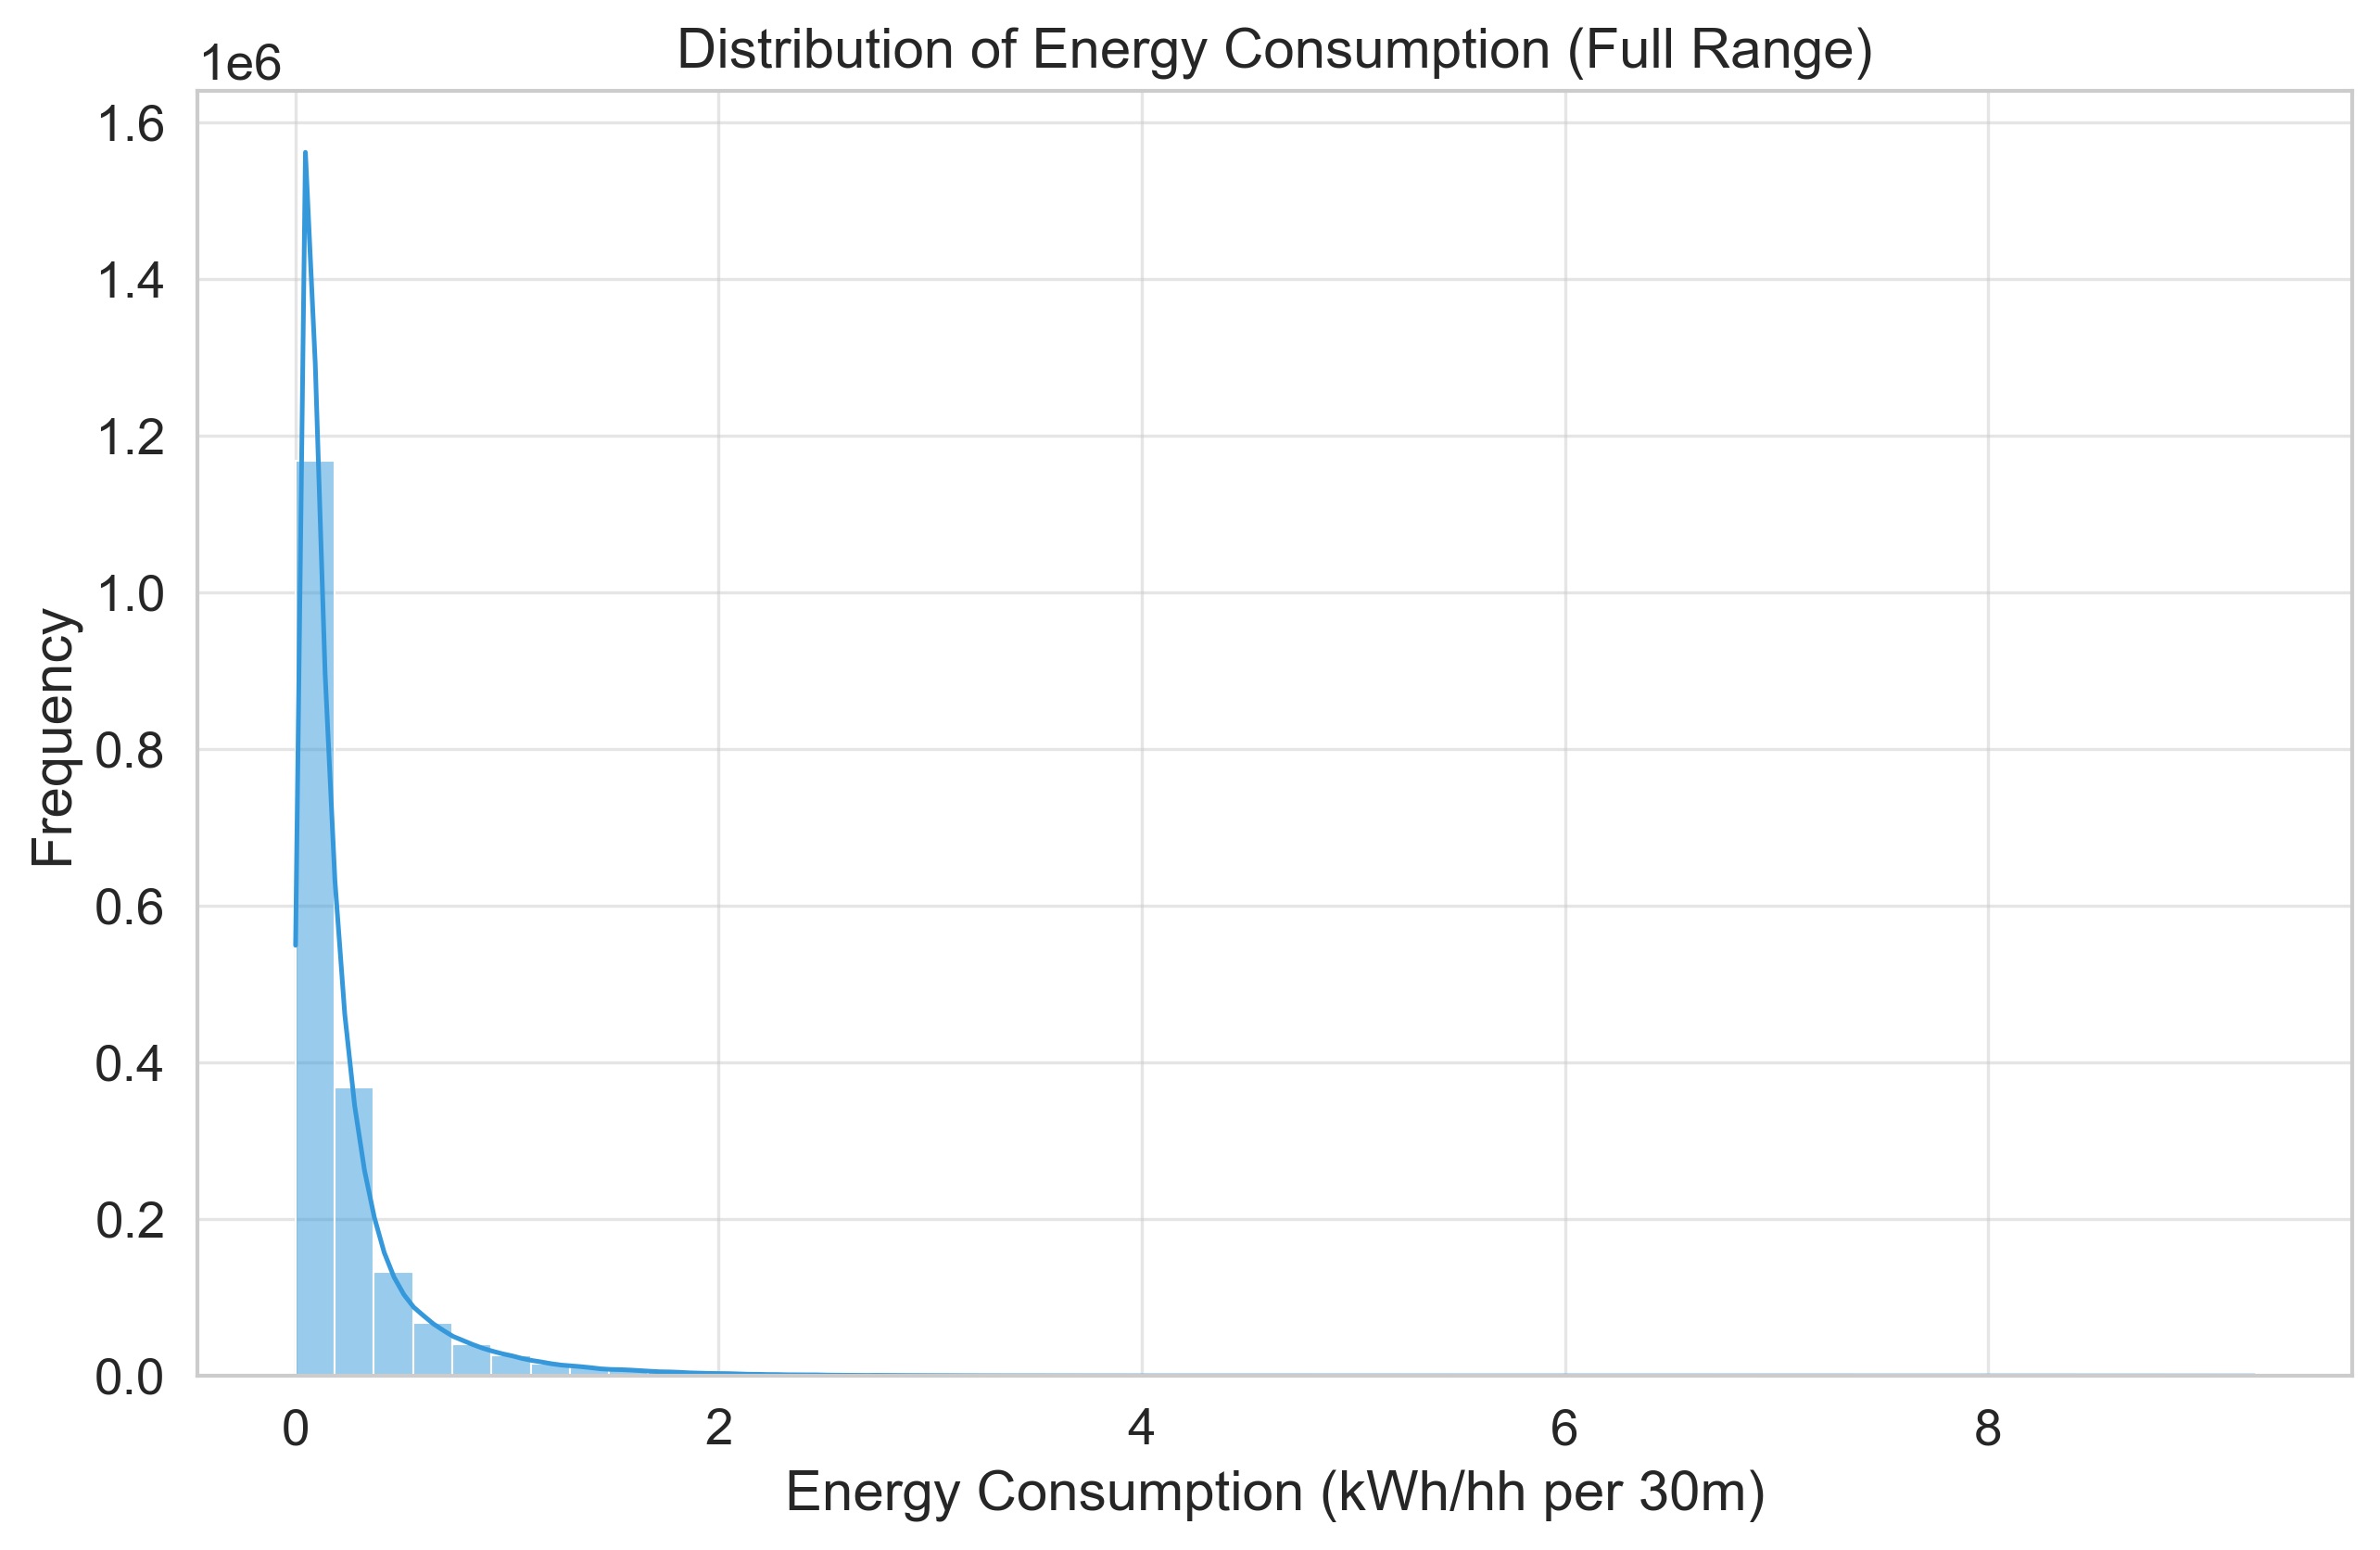
\includegraphics[width=1\textwidth]{figures/distribution_full_range.png}
    \caption{Distribution of raw energy consumption (Scientific Notation).}
    \label{fig:dist_full}
\end{figure}


To better understand the behavior of the majority of the population, Figure \ref{fig:dist_zoomed} provides a focused view of the 0.0 to 1.0 kWh range. This interval is highly significant as it contains approximately 96.5\% of all recorded tuples collected across the entire one-week observation period (336 snapshots) defined in Section~\ref{sec:dataset}. 

\begin{figure}[thp]
    \centering
    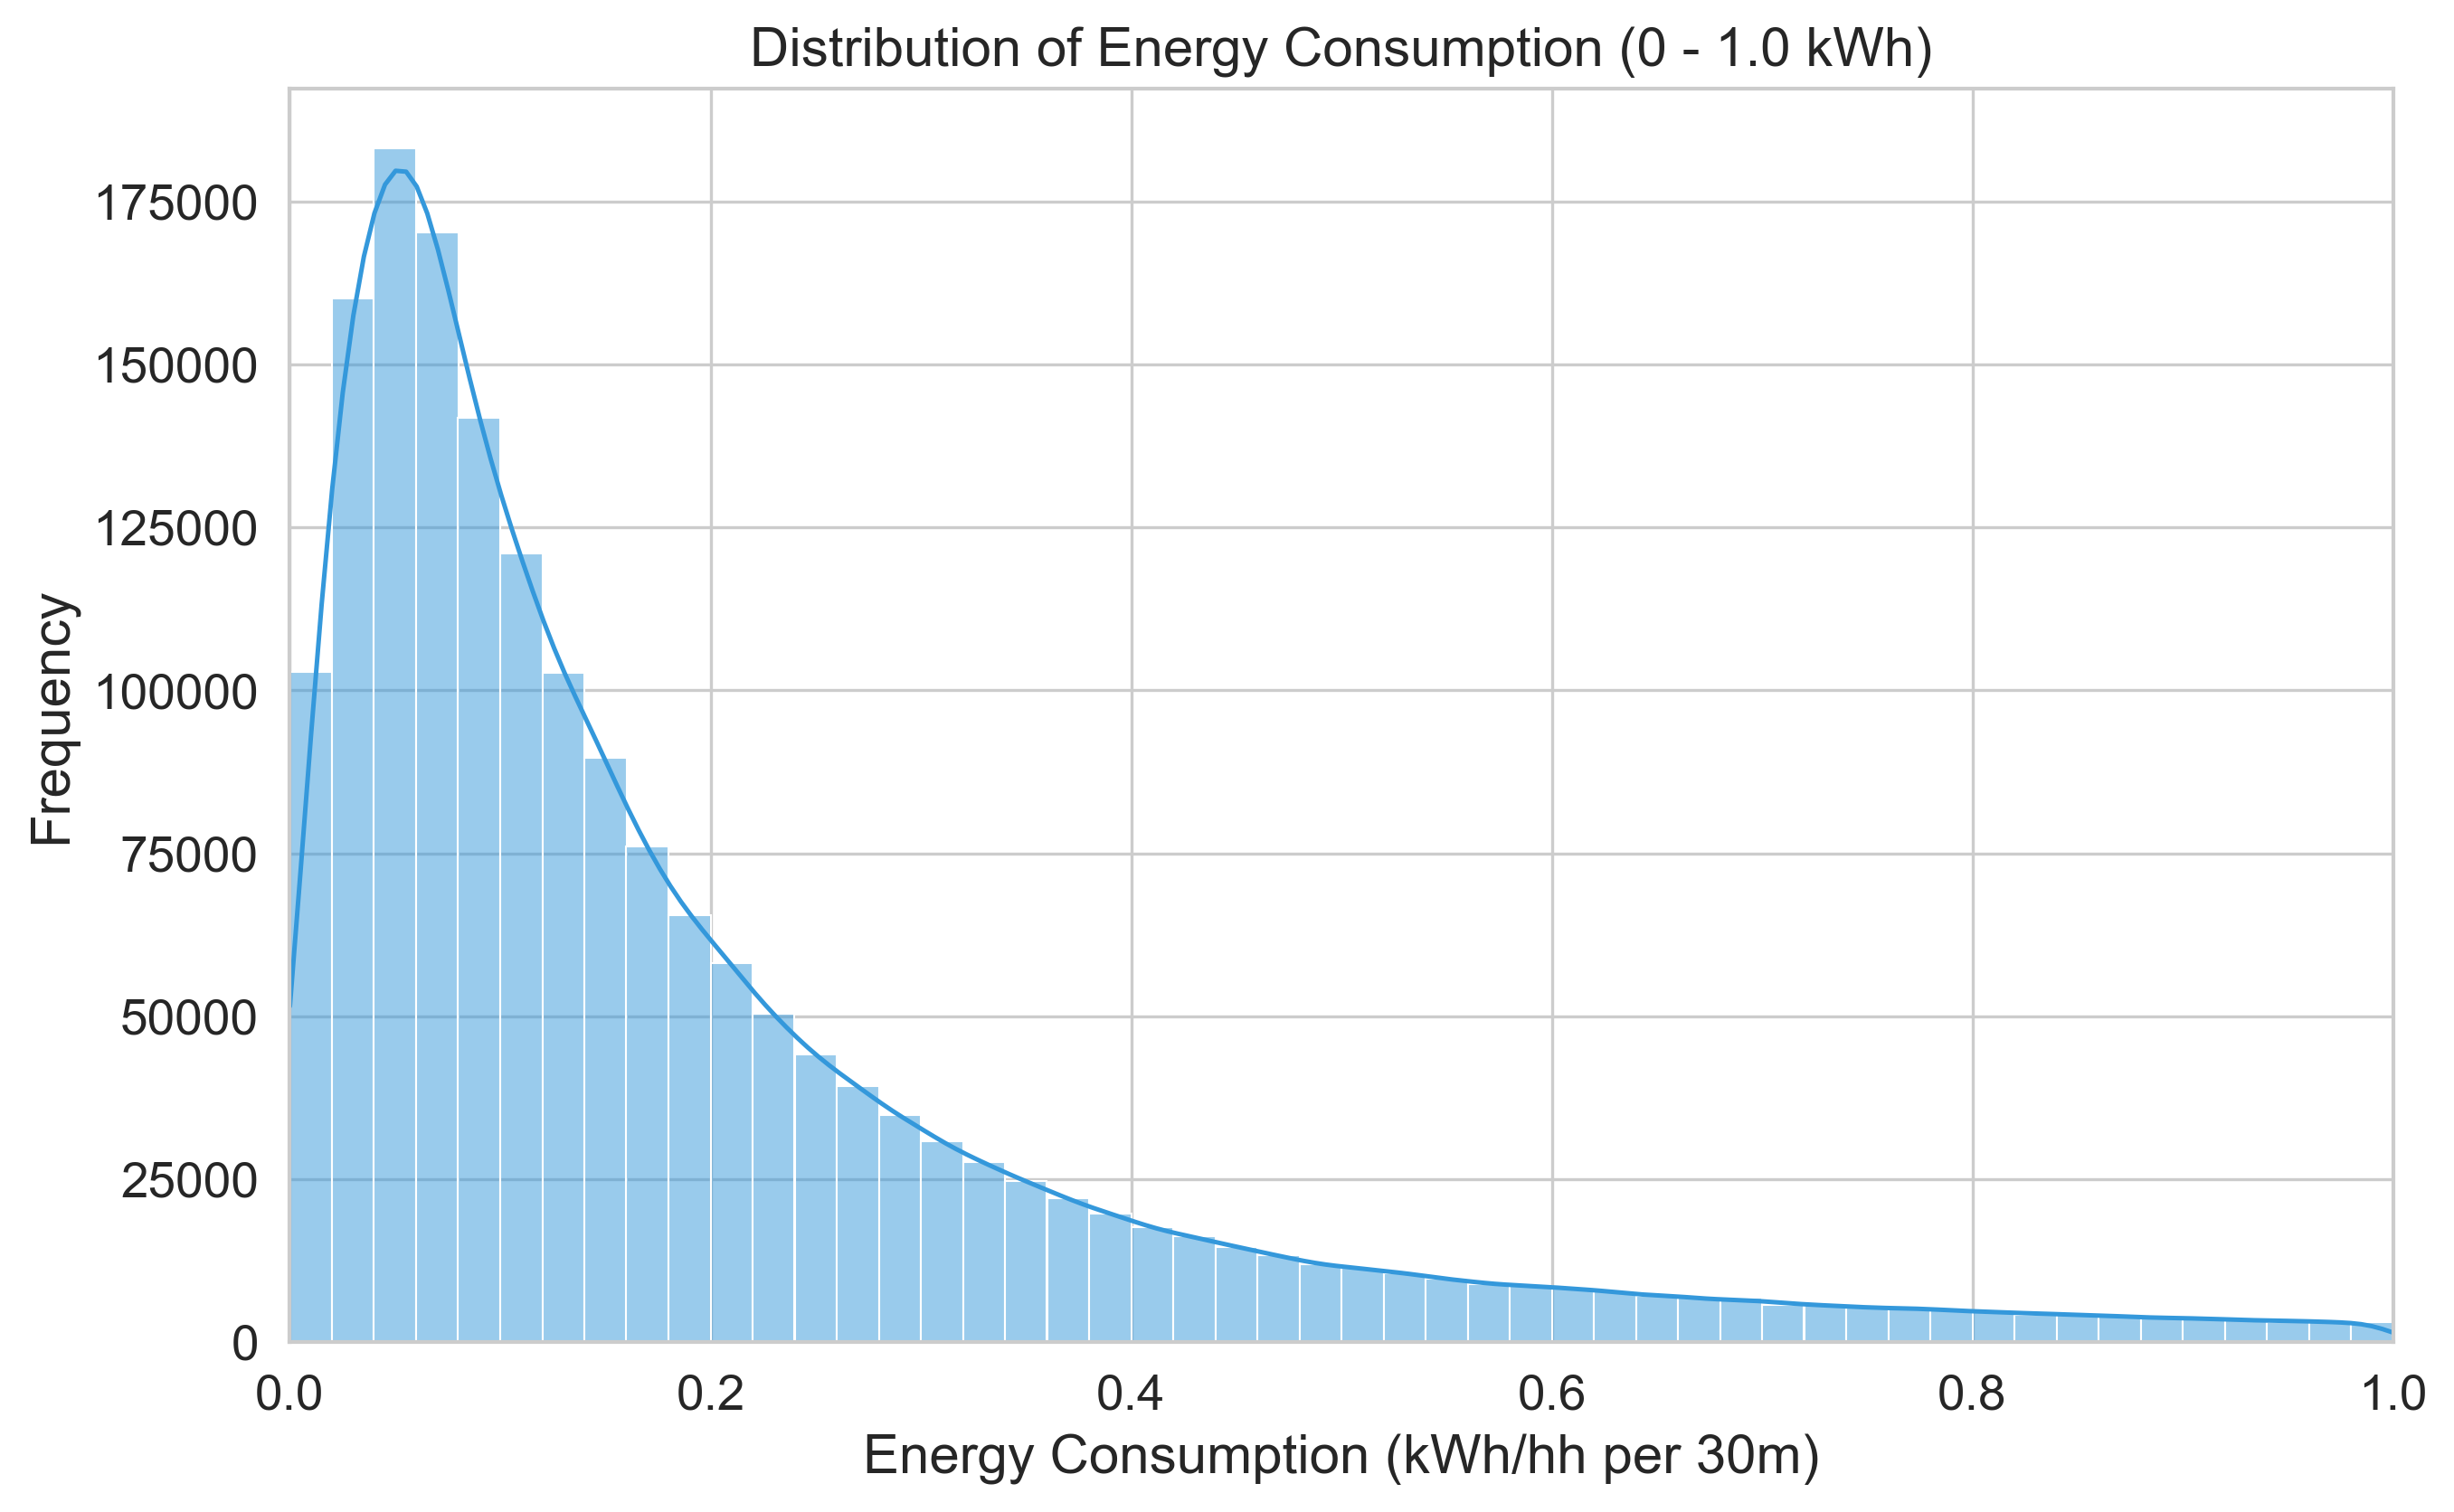
\includegraphics[width=1\textwidth]{figures/distribution_zoomed_to_1kwh.png}
    \caption{Detailed view of the 0-1.0 kWh range, representing 96.5\% of the total population data aggregated over the full one-week duration (Nov 5-11, 2012).}
    \label{fig:dist_zoomed}
\end{figure}

The distribution reveals two primary characteristics:
\begin{enumerate}
    \item \textbf{Low-Load Concentration:} A significant majority of readings are clustered between 0 kWh and 0.2 kWh. In this range, the high density of users suggests a higher probability of satisfying $z$-anonymity thresholds.
    \item \textbf{High-Precision Sparsity:} Despite the apparent density of the low-load range, the data resolution results in a significant number of unique readings. While Figure~\ref{fig:dist_zoomed} shows that a bin at 0.6 kWh contains approximately 10,000 occurrences, this frequency must be interpreted within the temporal and numerical context of the snapshots. 

    First, these 10,000 occurrences are distributed across the entire one-week period, which consists of 336 distinct timestamps (7 days $\times$ 48 half-hour intervals). This results in an average of only $\approx 30$ tuples per bin per snapshot. Second, because each bin (0.02 kWh wide) encompasses 20 distinct measurement values due to the three-decimal-point precision (e.g., 0.600, 0.601, ..., 0.619), the 30 tuples are further fragmented. This results in an average of only \textbf{$\approx 1.5$ occurrences per specific raw value at any given timestamp}. Since $z$-anonymity requires a value to appear at least $z$ times to satisfy the anonymity threshold, the raw high-precision data is effectively "near zero" in terms of publishable frequency. This sparsity at the individual measurement level is the primary driver of the near-total suppression observed in the global \textbf{Baseline performance}, which is further analyzed in Section~\ref{sec:baseline} (Figure~\ref{fig:baseline}).

\end{enumerate}




While the histograms characterize the range of values, energy consumption is inherently temporal. To understand the privacy challenges in a streaming context, we must analyze how user behavior and data sparsity evolve over a daily cycle. Figure \ref{fig:daily_load_sparsity} illustrates the relationship between average consumption and the uniqueness of the data.

As shown in Figure \ref{fig:load_profile}, the dataset exhibits the standard "double-peak" characteristic of residential demand, with a minor morning peak at 08:30 and a major evening peak lasting from 16:00 to 22:00. Figure \ref{fig:sparsity_trend} reveals that the number of unique energy readings follows this consumption curve almost perfectly. 

During the evening peak, the count of unique values rises to approximately 1,250 per snapshot. Within a population of 5,529 users, this indicates that nearly one out of every four users reports a value that is unique to three decimal places during high-activity periods. In contrast, during the early morning hours (02:00--05:00), the number of unique values drops to approximately 580, suggesting a much higher concentration of identical readings during low-load periods. 

The heatmap in Figure \ref{fig:dist_heatmap} confirms that these patterns are consistent across the selected week. While the morning peak shifts slightly during the weekend (Saturday and Sunday), the high entropy associated with evening usage remains a constant characteristic of the dataset.
% \clearpage % images finished before starting the next section 
\begin{figure}[H]
\centering
\begin{subfigure}{0.80\textwidth}
\centering
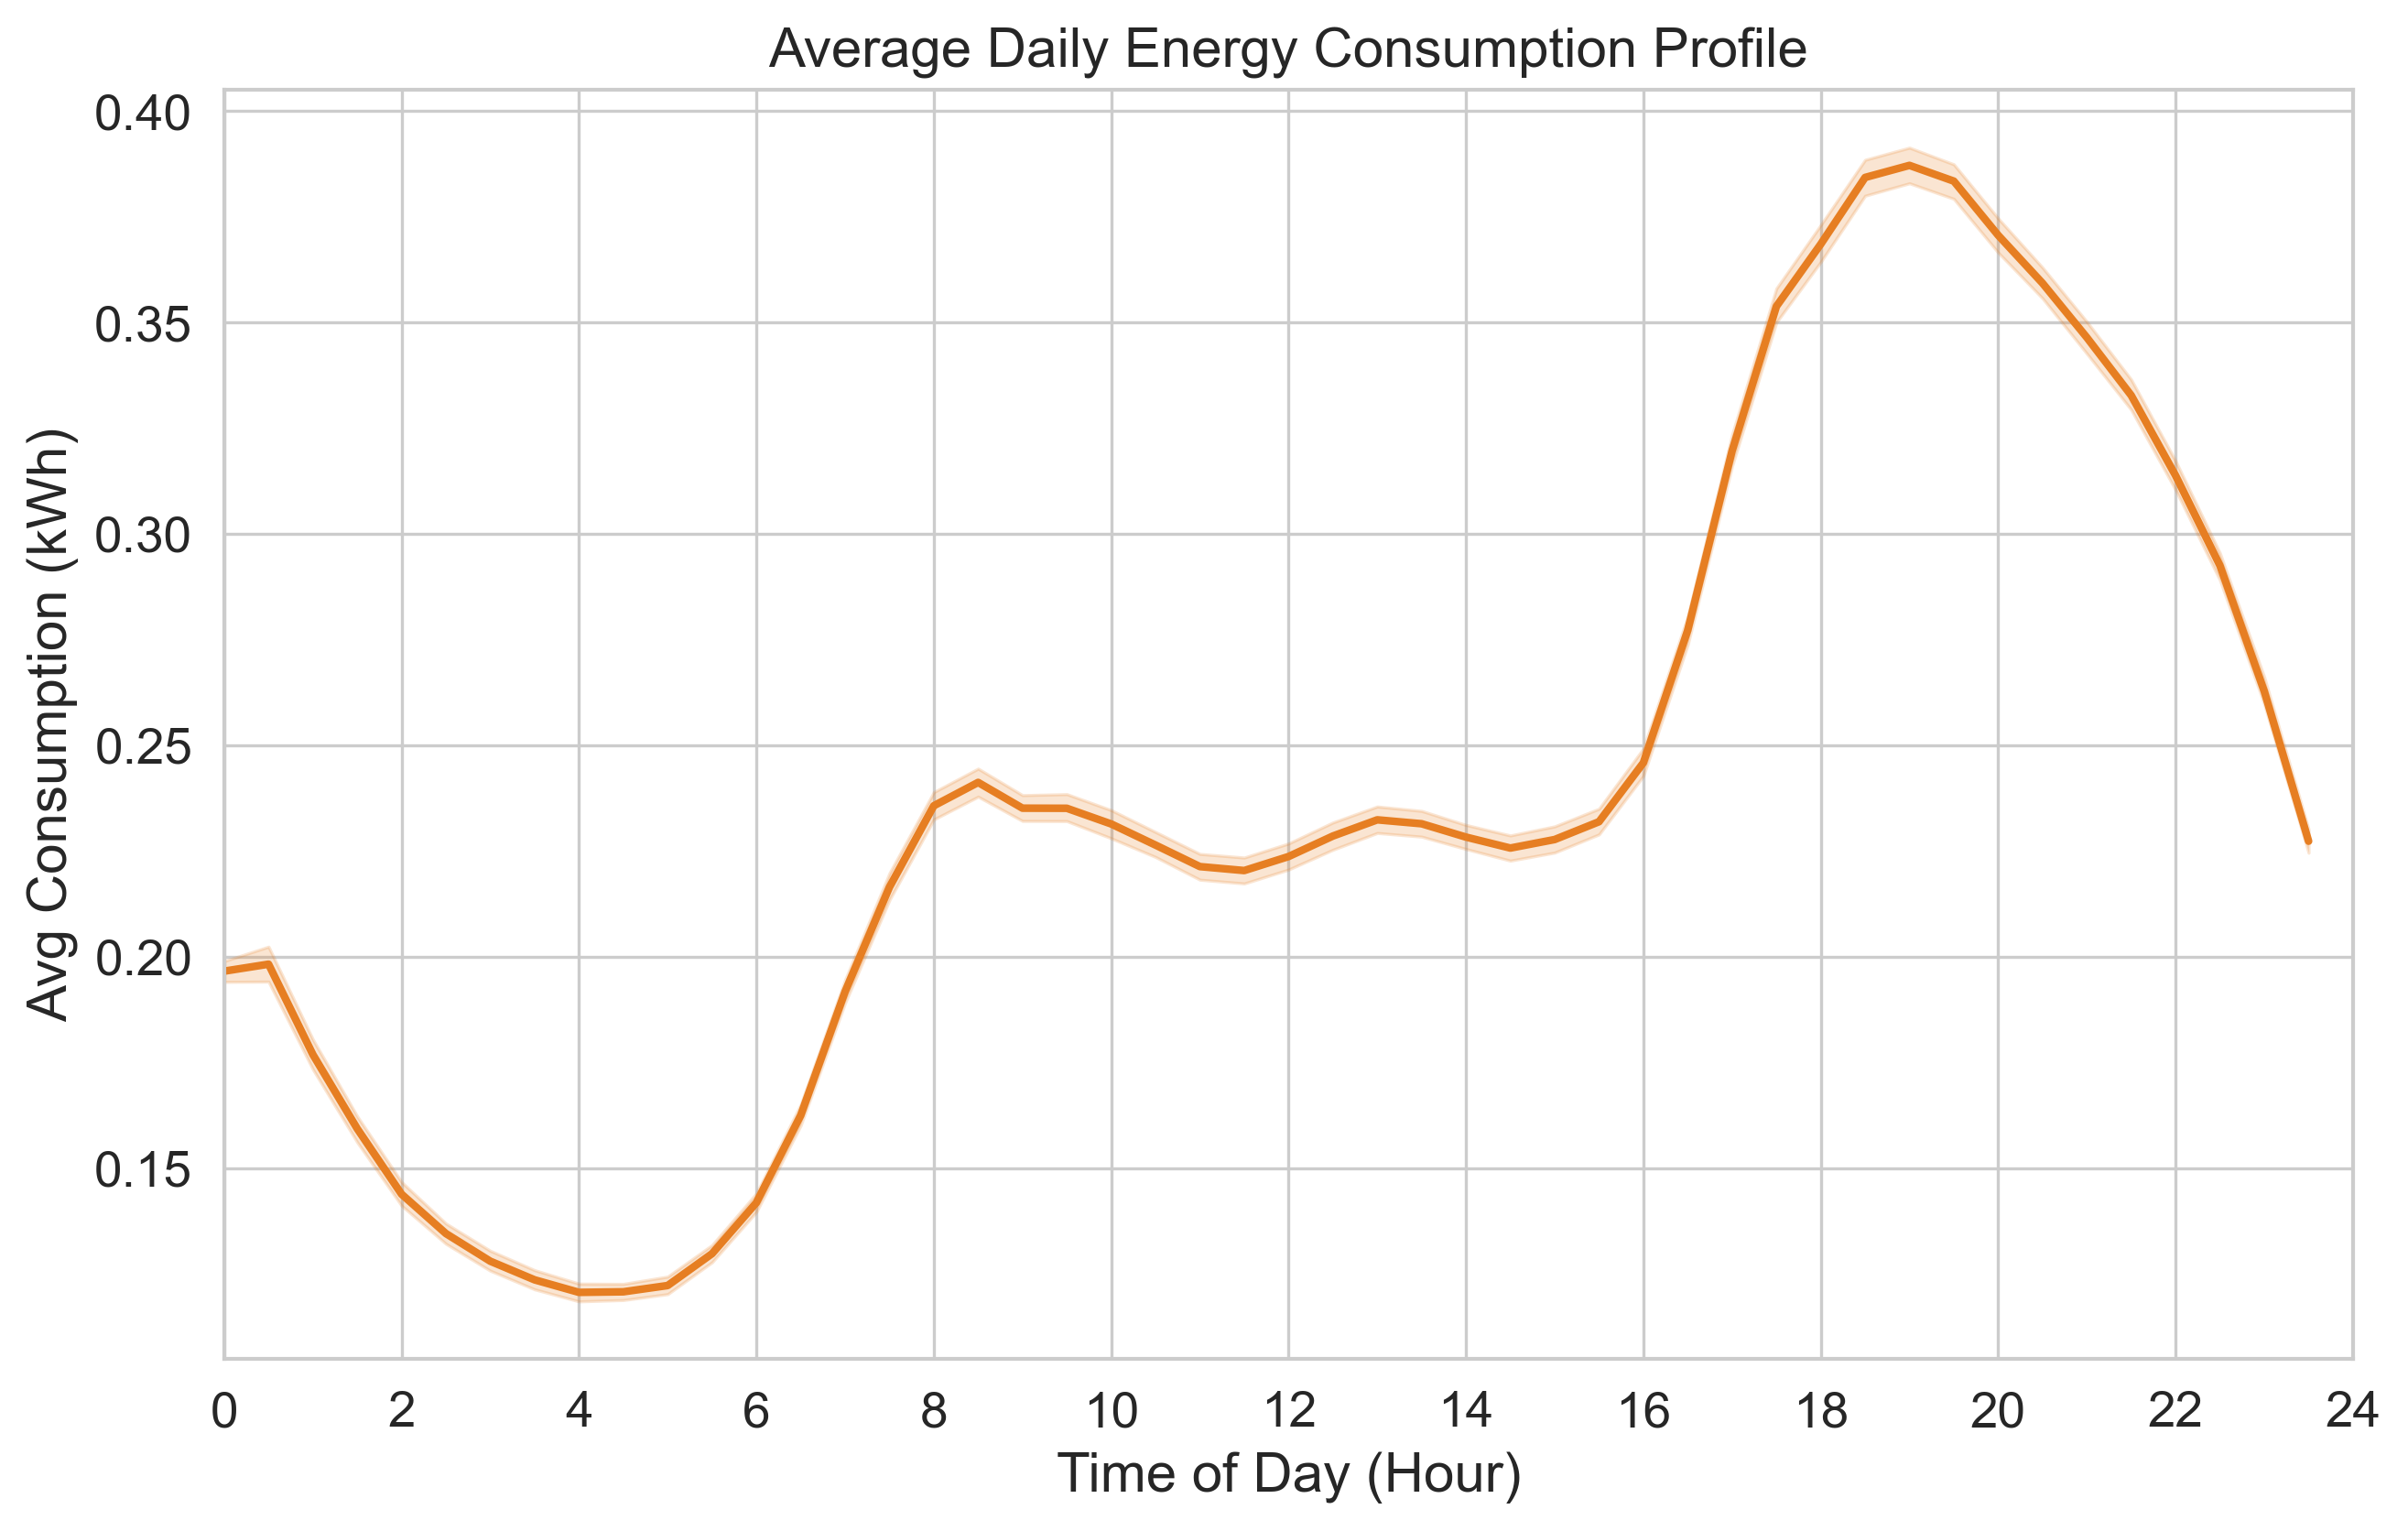
\includegraphics[width=\textwidth]{figures/distribution_daily_profile.png}
\caption{Average Daily Load Profile.}
\label{fig:load_profile}
\end{subfigure}
\hfill
\begin{subfigure}{0.80\textwidth}
\centering
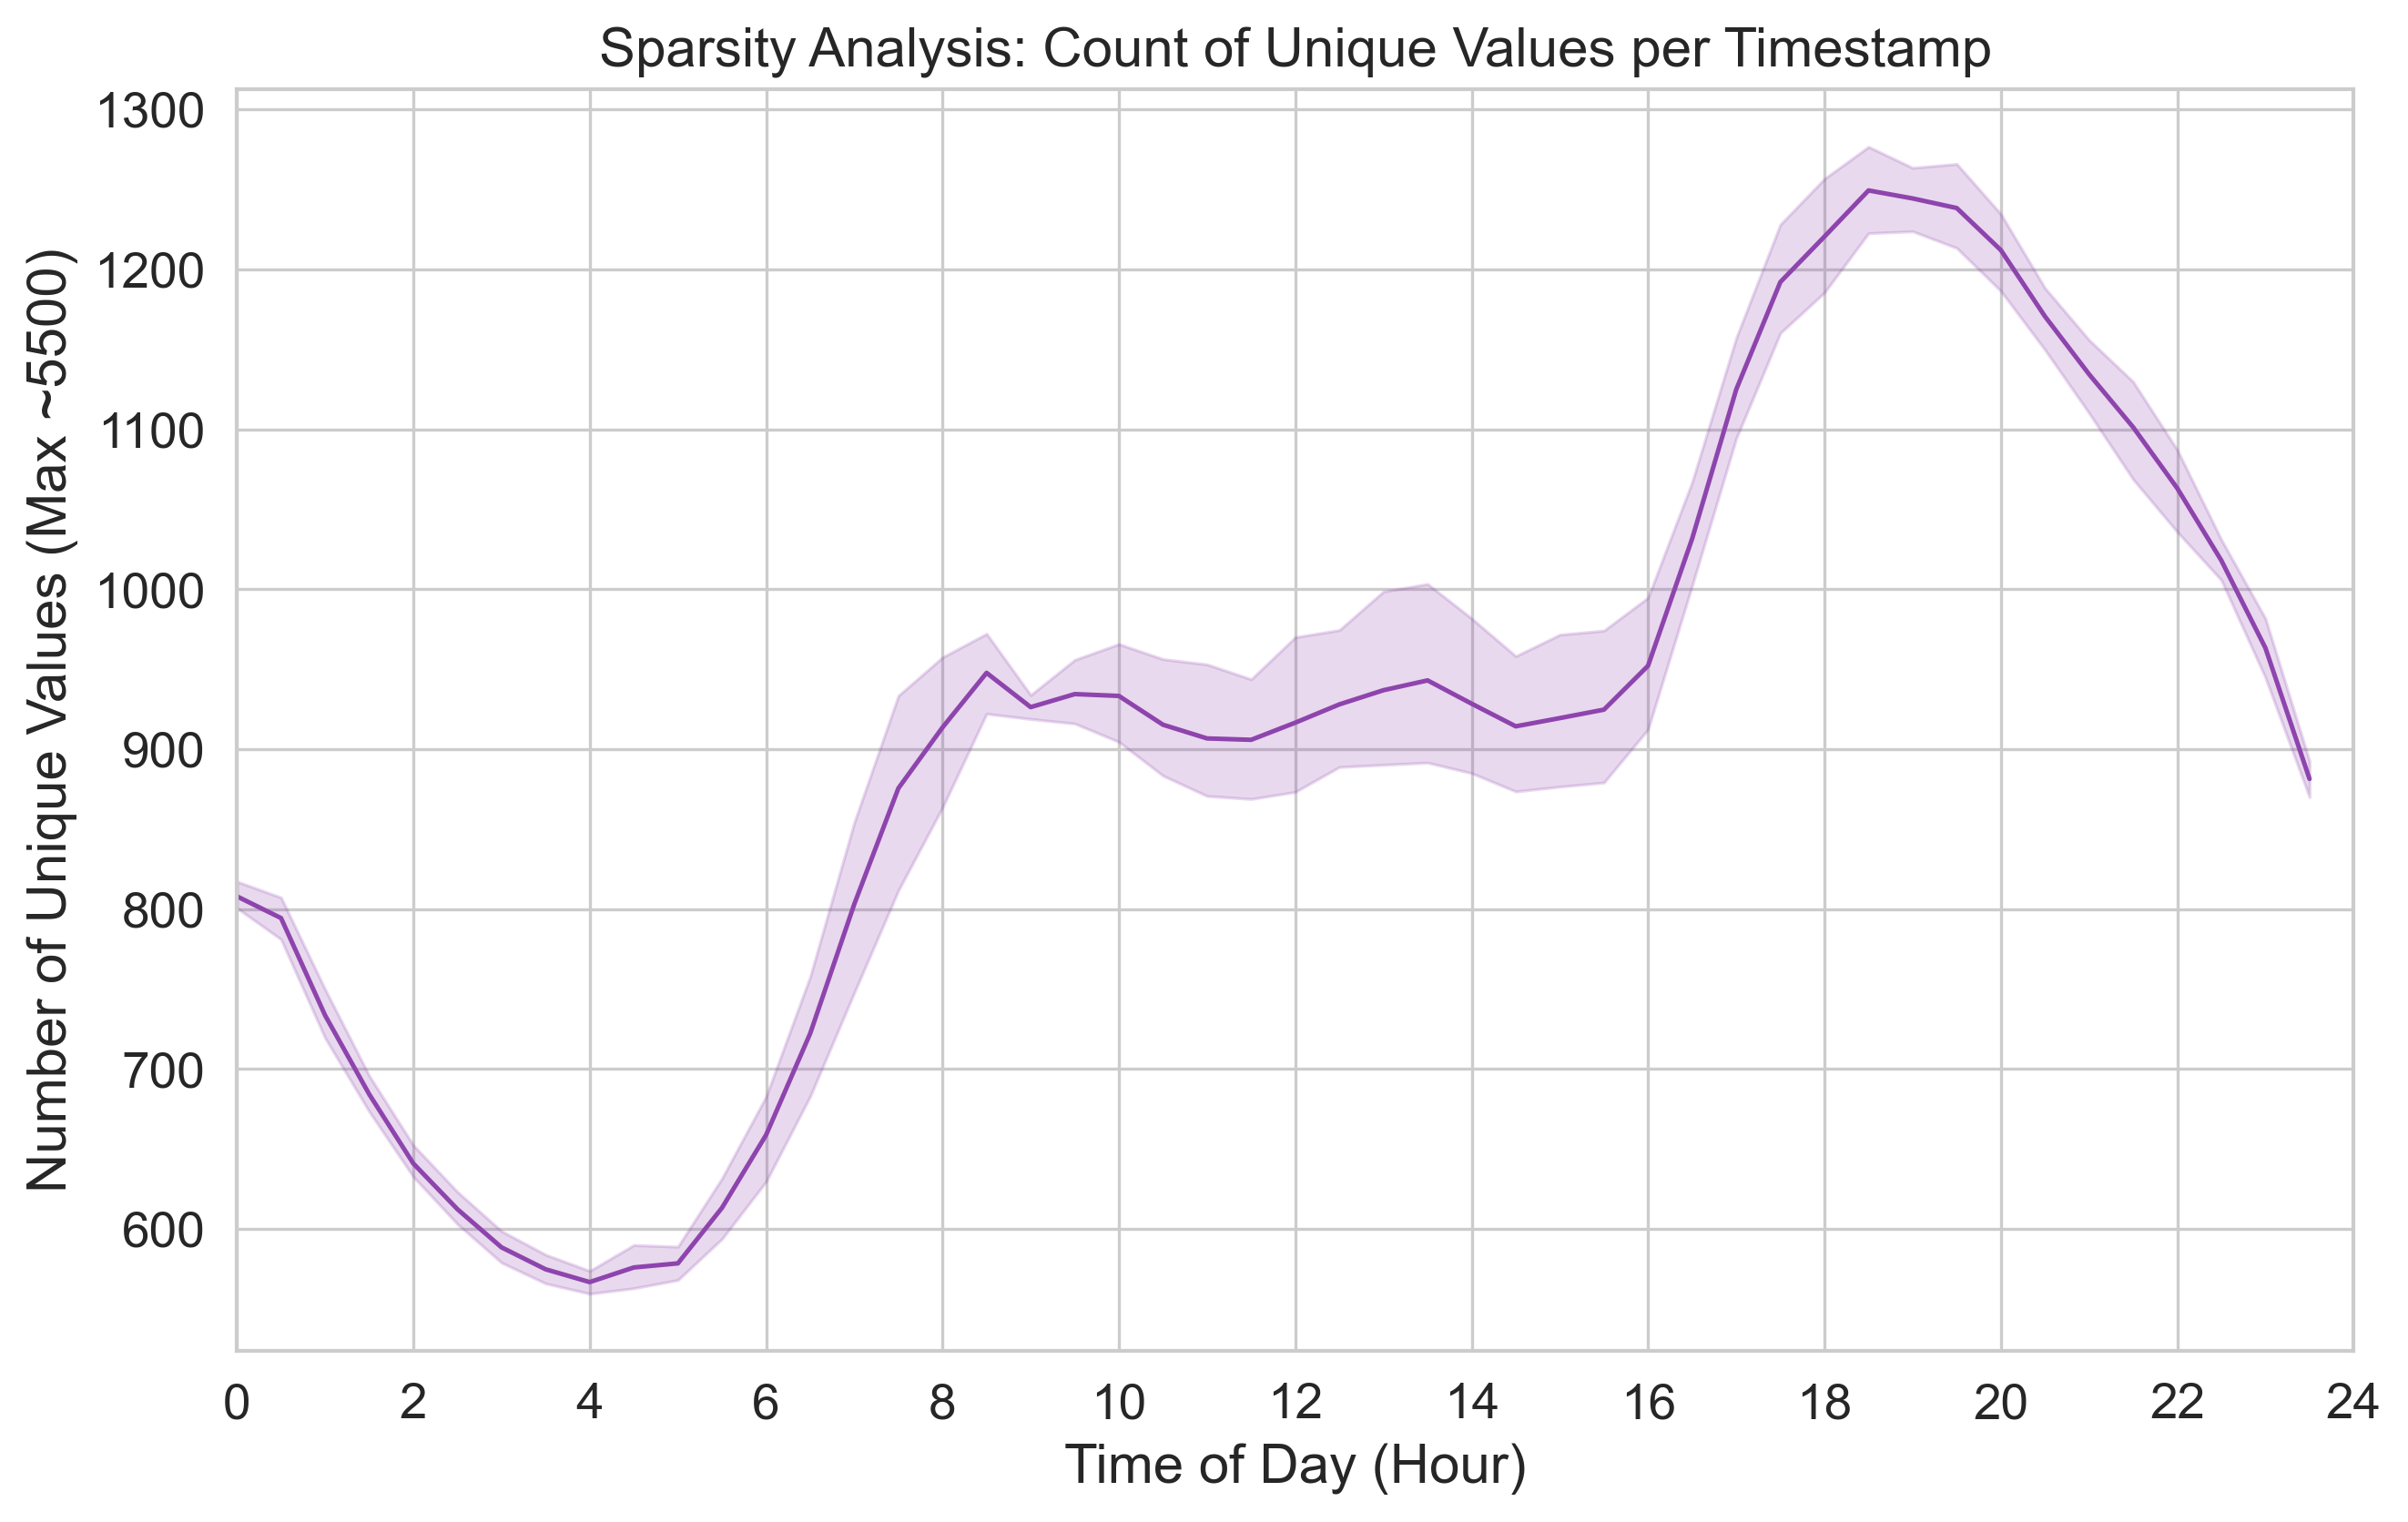
\includegraphics[width=\textwidth]{figures/distribution_sparsity.png}
\caption{Count of Unique Values per Timestamp.}
\label{fig:sparsity_trend}
\end{subfigure}
\hfill
\begin{subfigure}{0.80\textwidth}
\centering
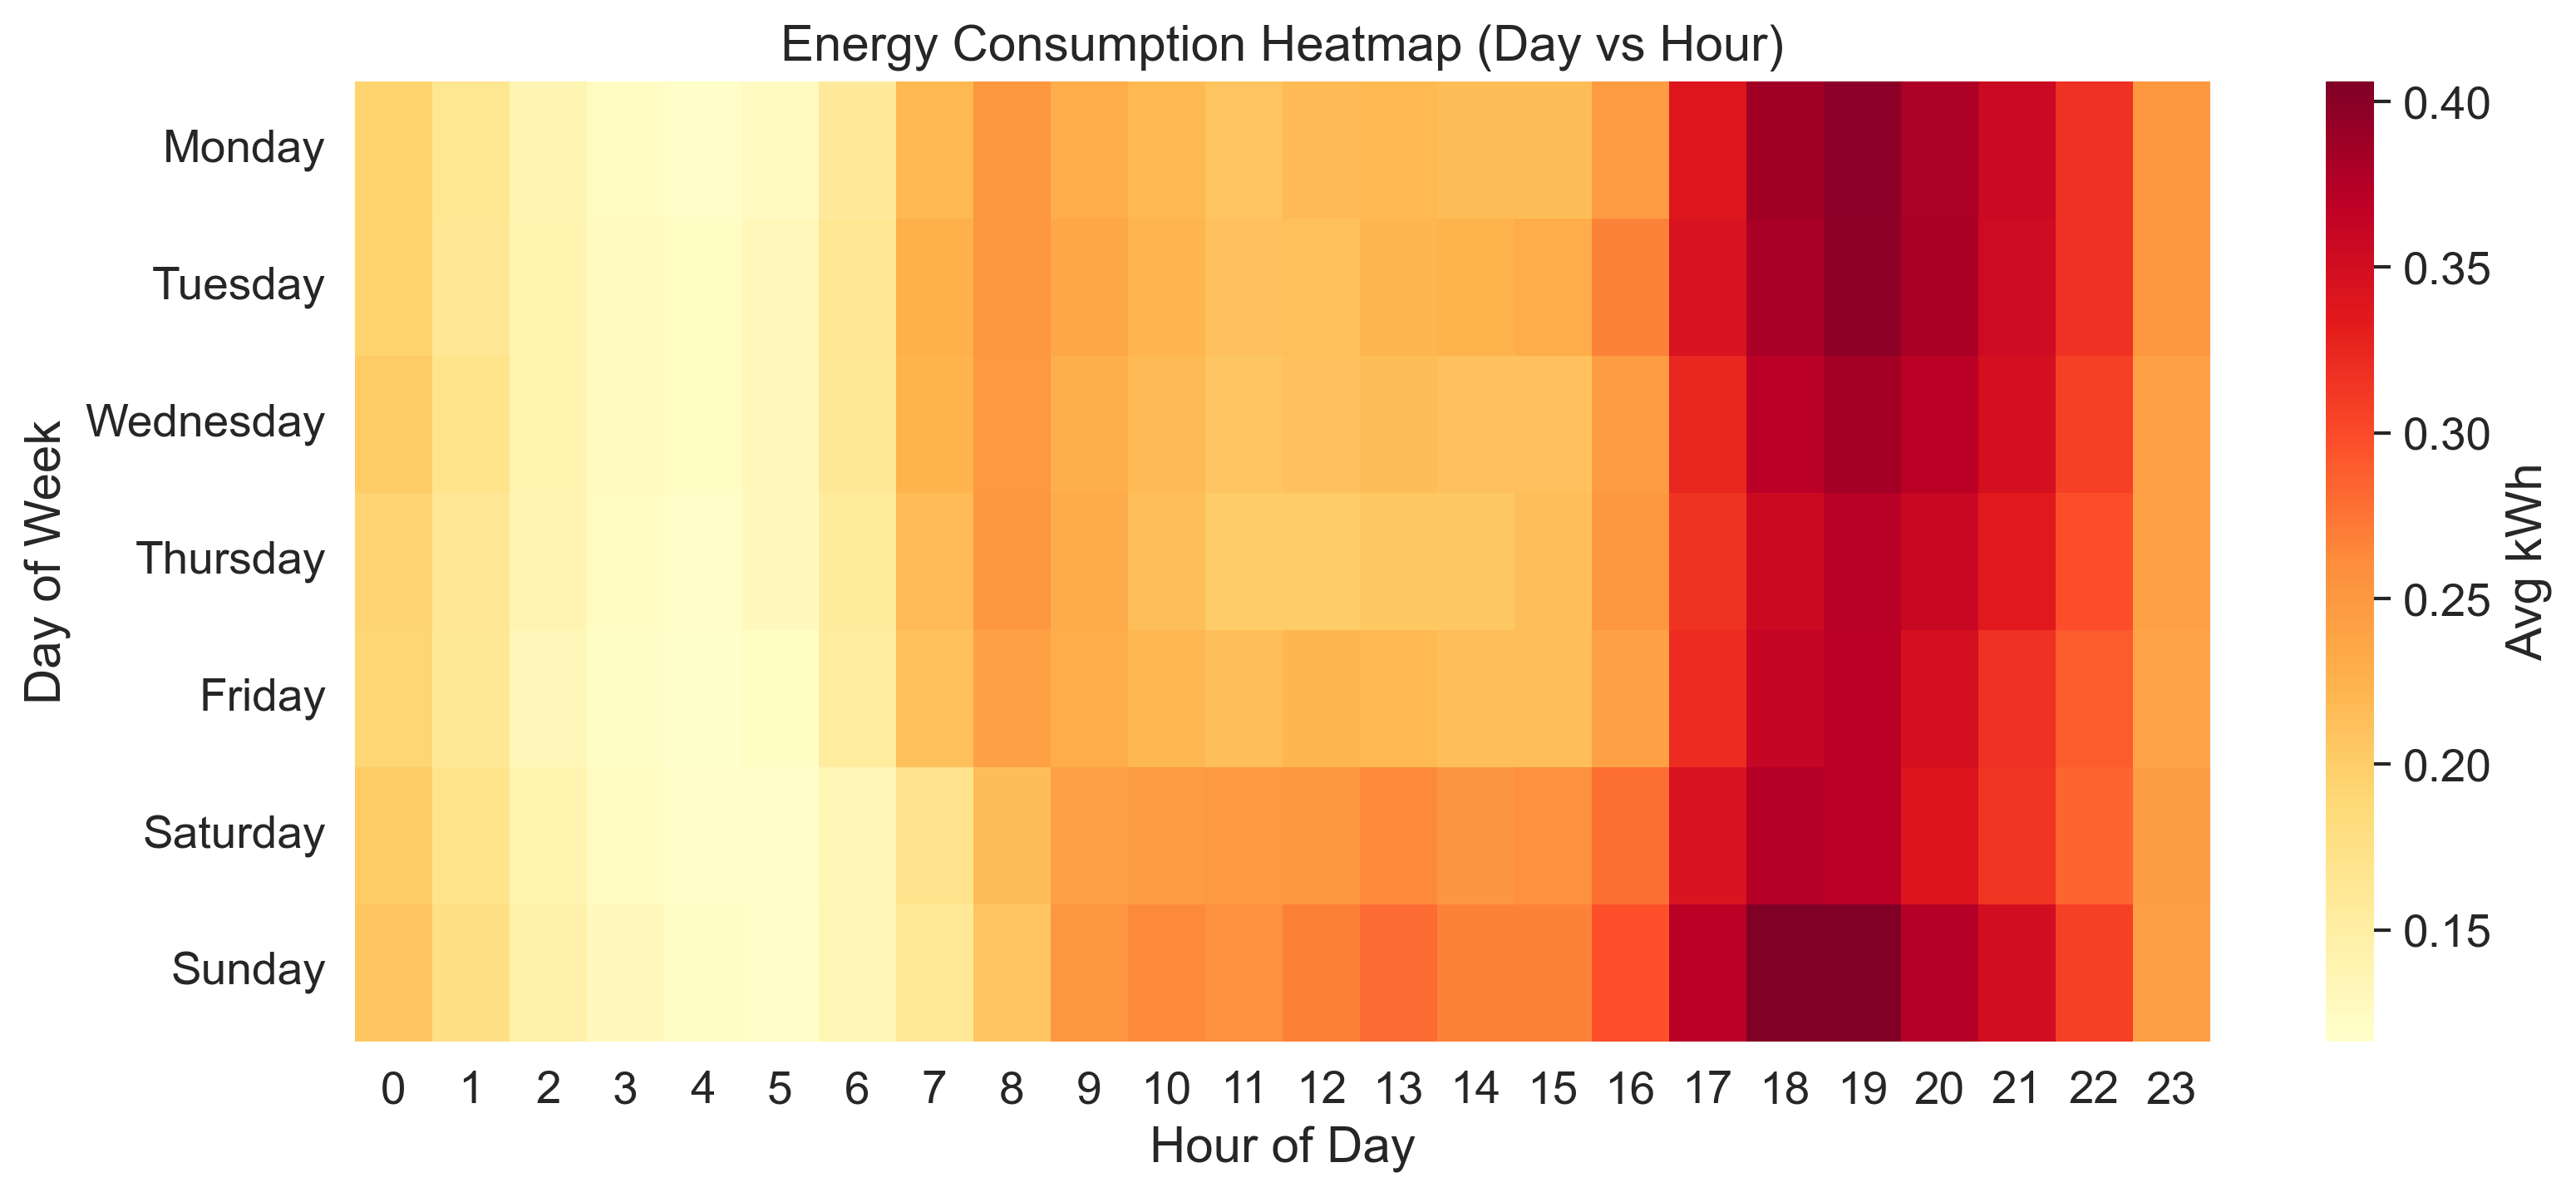
\includegraphics[width=\textwidth]{figures/distribution_heatmap.png}
\caption{Heatmap of energy consumption across the week.}
\label{fig:dist_heatmap}
\end{subfigure}
\caption{Temporal analysis of the dataset over a 24-hour cycle.}
\label{fig:daily_load_sparsity}
\end{figure}


% As shown in Figure \ref{fig:load_profile}, the dataset exhibits the standard "double-peak" characteristic of residential demand, with a minor morning peak at 08:30 and a major evening peak lasting from 16:00 to 22:00. Figure \ref{fig:sparsity_trend} reveals that the number of unique energy readings follows this consumption curve almost perfectly. 

% During the evening peak, the count of unique values rises to approximately 1,250 per snapshot. Within a population of 5,529 users, this indicates that nearly one out of every four users reports a value that is unique to three decimal places during high-activity periods. In contrast, during the early morning hours (02:00--05:00), the number of unique values drops to approximately 580, suggesting a much higher concentration of identical readings during low-load periods. 

% The heatmap in Figure \ref{fig:dist_heatmap} confirms that these patterns are consistent across the selected week. While the morning peak shifts slightly during the weekend (Saturday and Sunday), the high entropy associated with evening usage remains a constant characteristic of the dataset.

% \begin{figure}[H]
% \centering
% 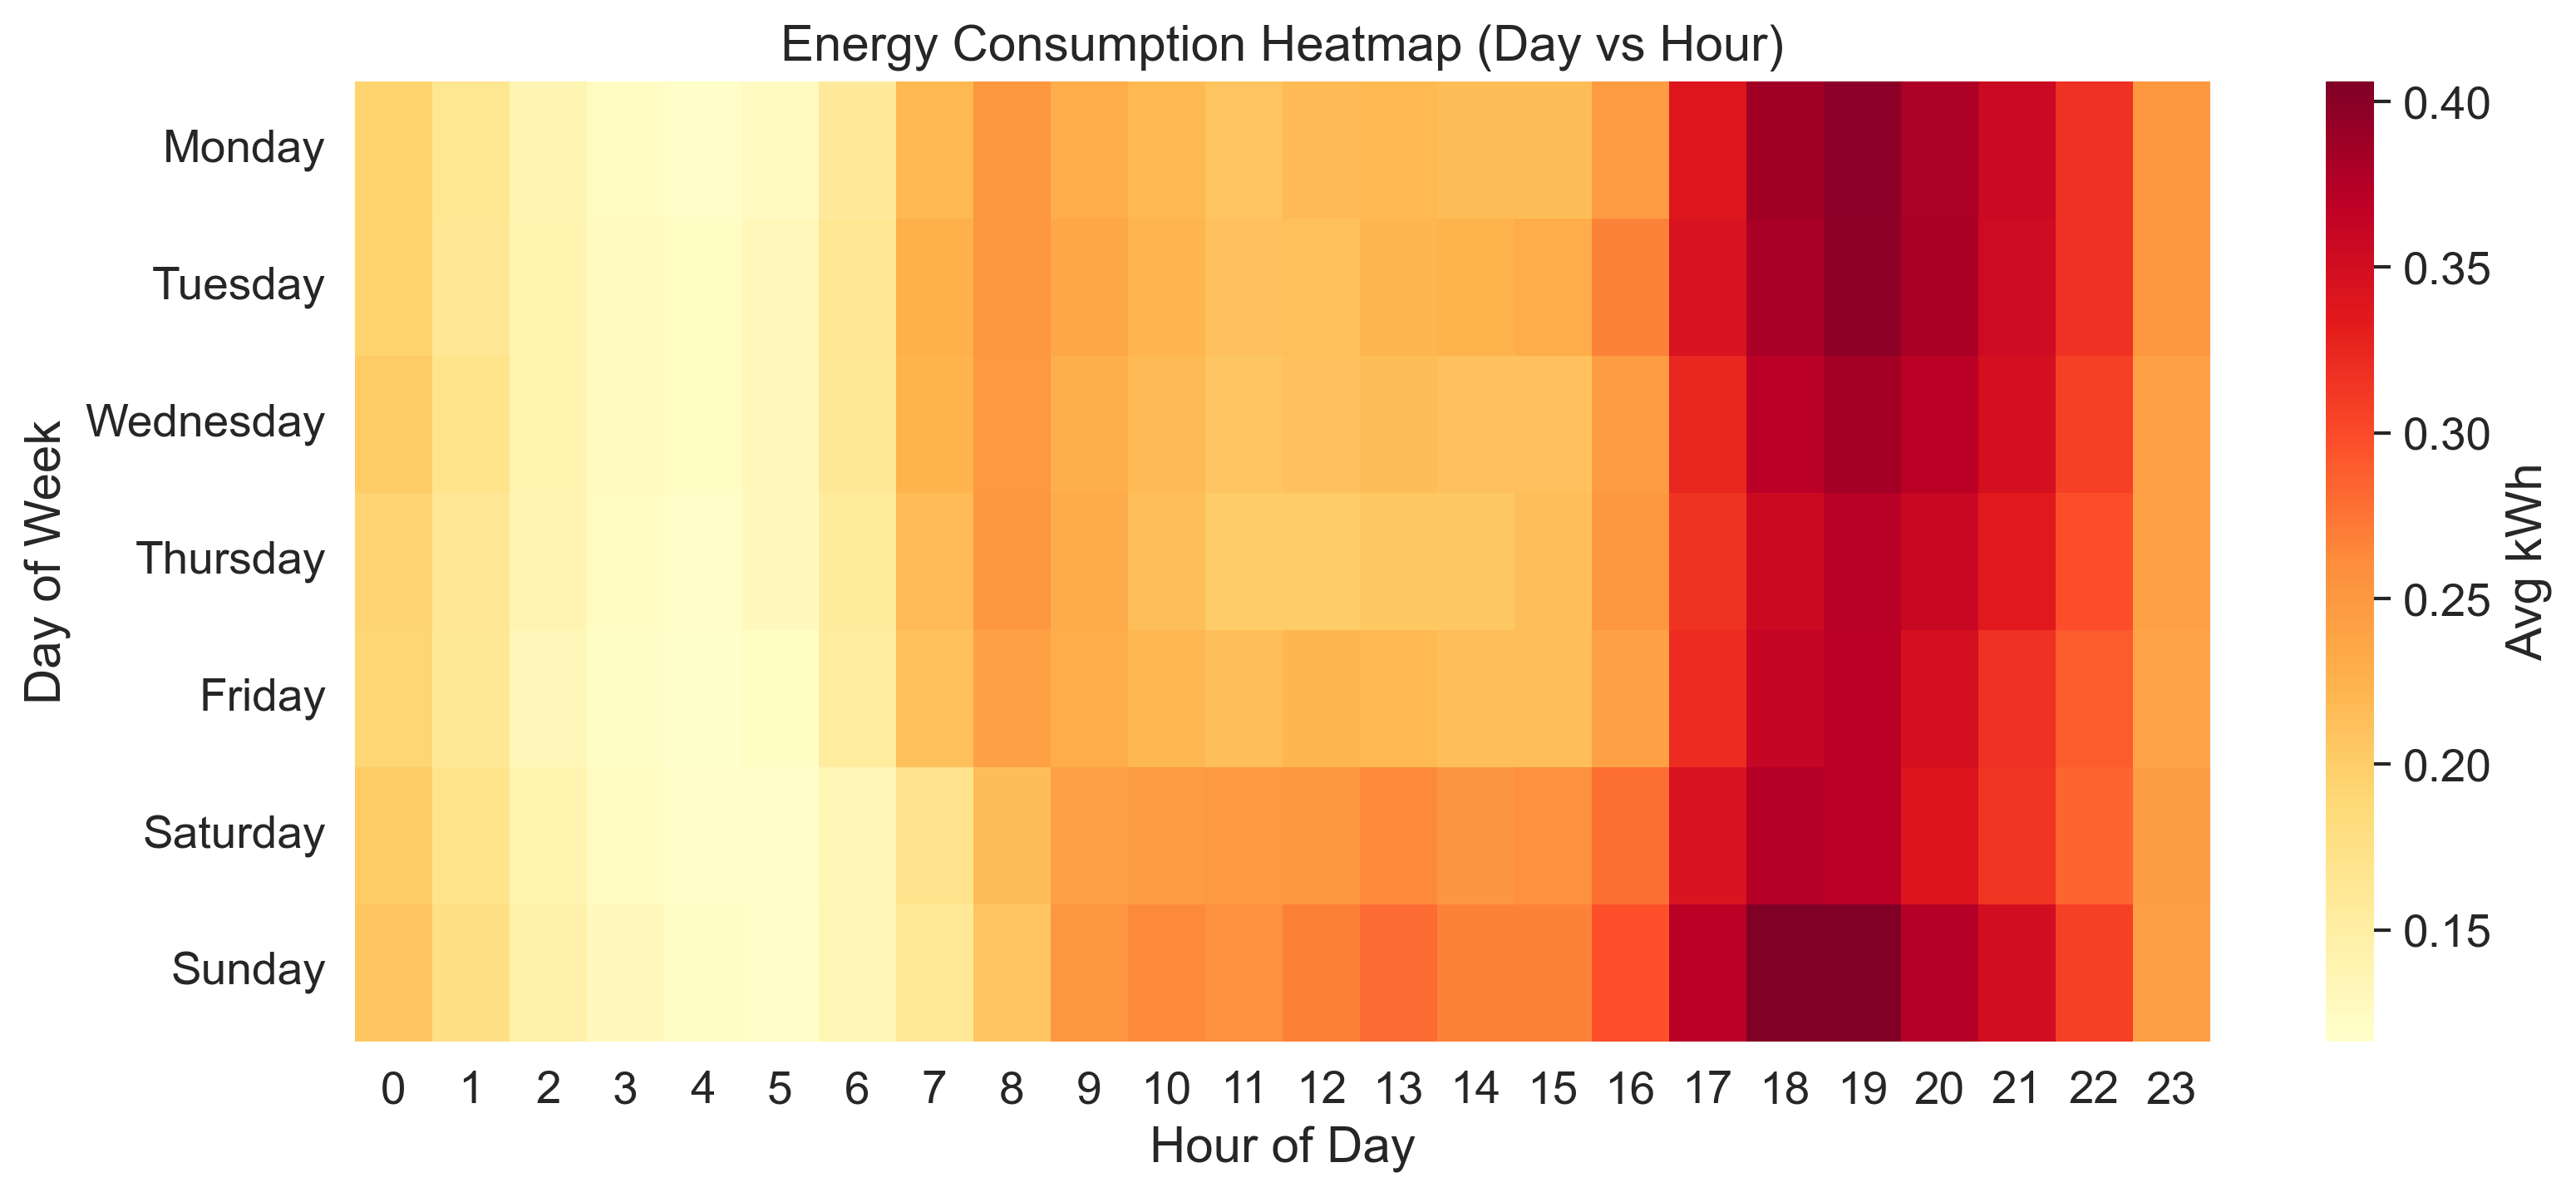
\includegraphics[width=0.9\textwidth]{figures/distribution_heatmap.png}
% \caption{Heatmap of energy consumption across the week.}
% \label{fig:dist_heatmap}
% \end{figure}

\section{Baseline Performance (Cloud-Only)}
\label{sec:baseline}
The Baseline scenario represents the centralized approach where raw data is transmitted directly to the Cloud before the privacy check is applied. This serves as the control group for the experiments.

Figure \ref{fig:baseline} depicts the Publication Ratio as a function of the privacy threshold $z$. The results indicate a rapid degradation of data availability as the privacy requirement increases.

\begin{figure}[H]
    \centering
    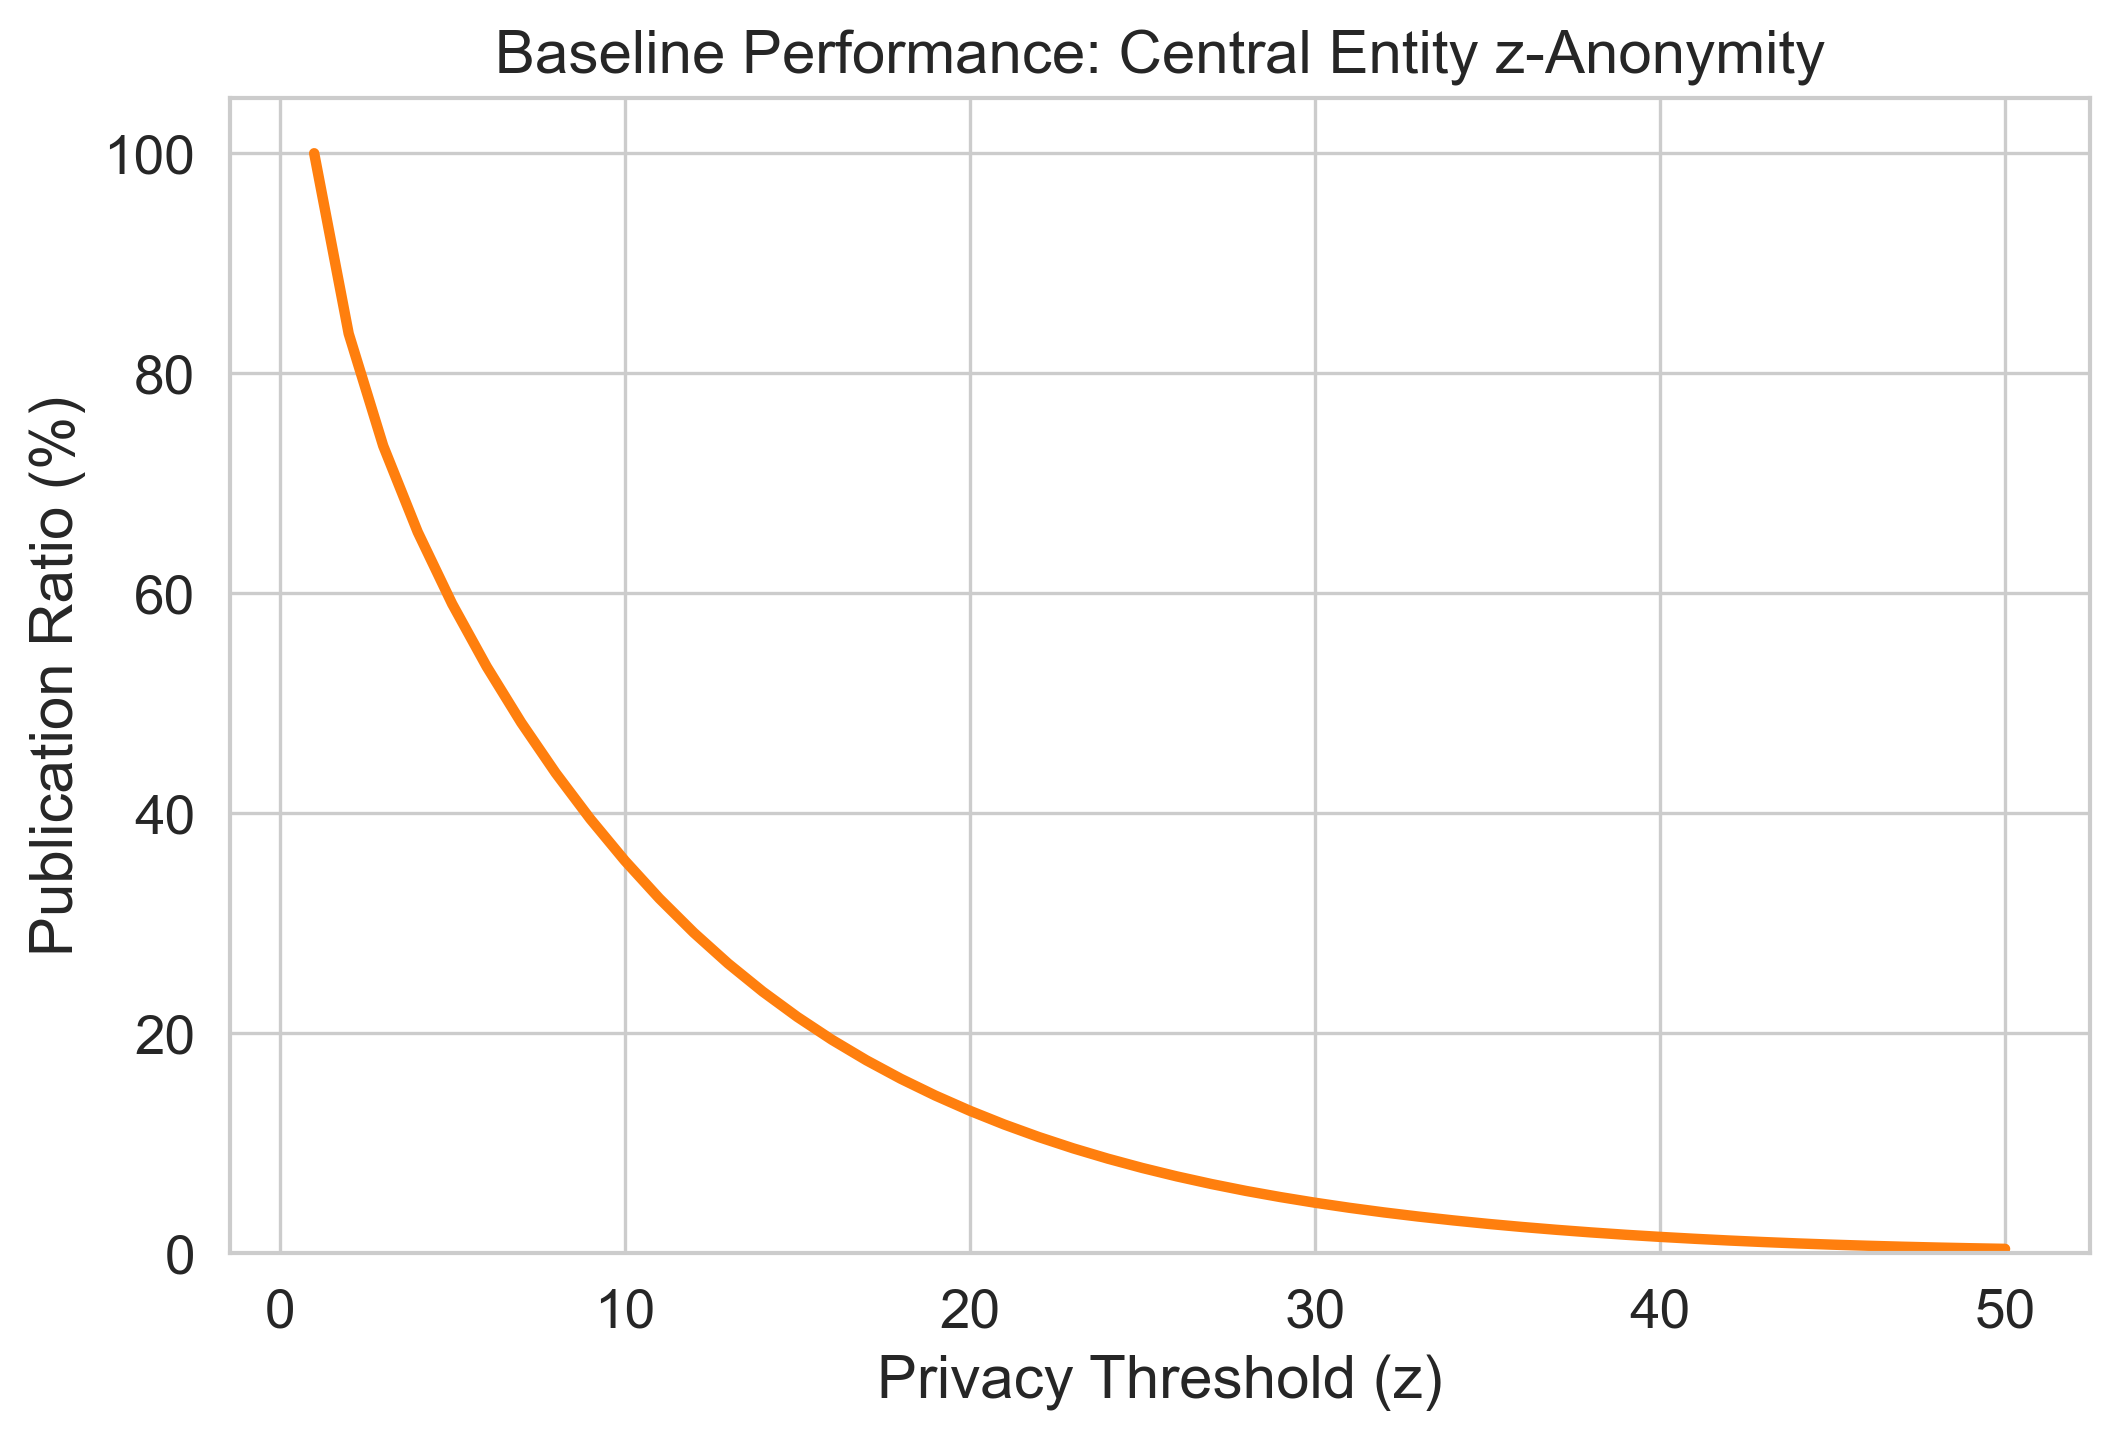
\includegraphics[width=0.82\textwidth]{figures/results_baseline.png}
    \caption{Baseline Performance: Publication Ratio vs. $z$.}
    \label{fig:baseline}
\end{figure}

Consistent with the sparsity observed in the data distribution analysis, the system struggles to maintain availability:
\begin{itemize}
    \item \textbf{At $z=2$:} The system publishes 83.6\% of the tuples.
    \item \textbf{At $z=10$:} The publication ratio drops to approximately 35.7\%.
    \item \textbf{At $z=50$:} The publication ratio falls below 0.4\%.
\end{itemize}

Given the total population of 5,529 households, finding at least two matching consumption readings at a single timestamp is statistically probable, especially within the low-load ranges identified in Section~\ref{sec:datadistribution}. This explains the relatively high data availability at $z=2$. However, as the threshold increases toward $z=50$, the high resolution of the raw data (three decimal places) makes it statistically improbable that 50 households will report the identical consumption value simultaneously. Consequently, the probability of satisfying a strict threshold like $z=50$ is near zero, leading to the near-total suppression of the dataset.


\section{Impact of Data Generalization}

The second experimental scenario evaluates the effectiveness of reducing numerical precision at the Edge Layer to improve the global publication ratio. The objective of this approach is to address the significant number of unique readings identified in the baseline analysis. By rounding energy consumption readings, we mathematically increase the probability that multiple users will report identical values within the same 30-minute snapshot, thereby facilitating the formation of the required "crowd" of size $z$.


Figure \ref{fig:results_gen_ratio} illustrates the publication ratio for three levels of precision ($p \in \{0, 1, 2\}$) compared against the high-precision Baseline ($p=3$).
The results demonstrate a dramatic improvement in data availability as data resolution is reduced:
\begin{itemize}
    \item \textbf{Precision 0 (Integer):} Provides the highest data availability, maintaining a publication ratio above 97\% across the entire tested range, including the strictest threshold of $z=50$.
    \item \textbf{Precision 1 (0.1 kWh):} Maintains a high publication ratio, staying above 87\% even at $z=50$, which indicates that most tuples successfully satisfy the privacy constraint at this resolution.
    \item \textbf{Precision 2 (0.01 kWh):} Shows a clear improvement over the high-precision Baseline but remains sensitive to the threshold; the publication ratio drops to 52\% at $z=50$.
\end{itemize}

\begin{figure}[H]
\centering
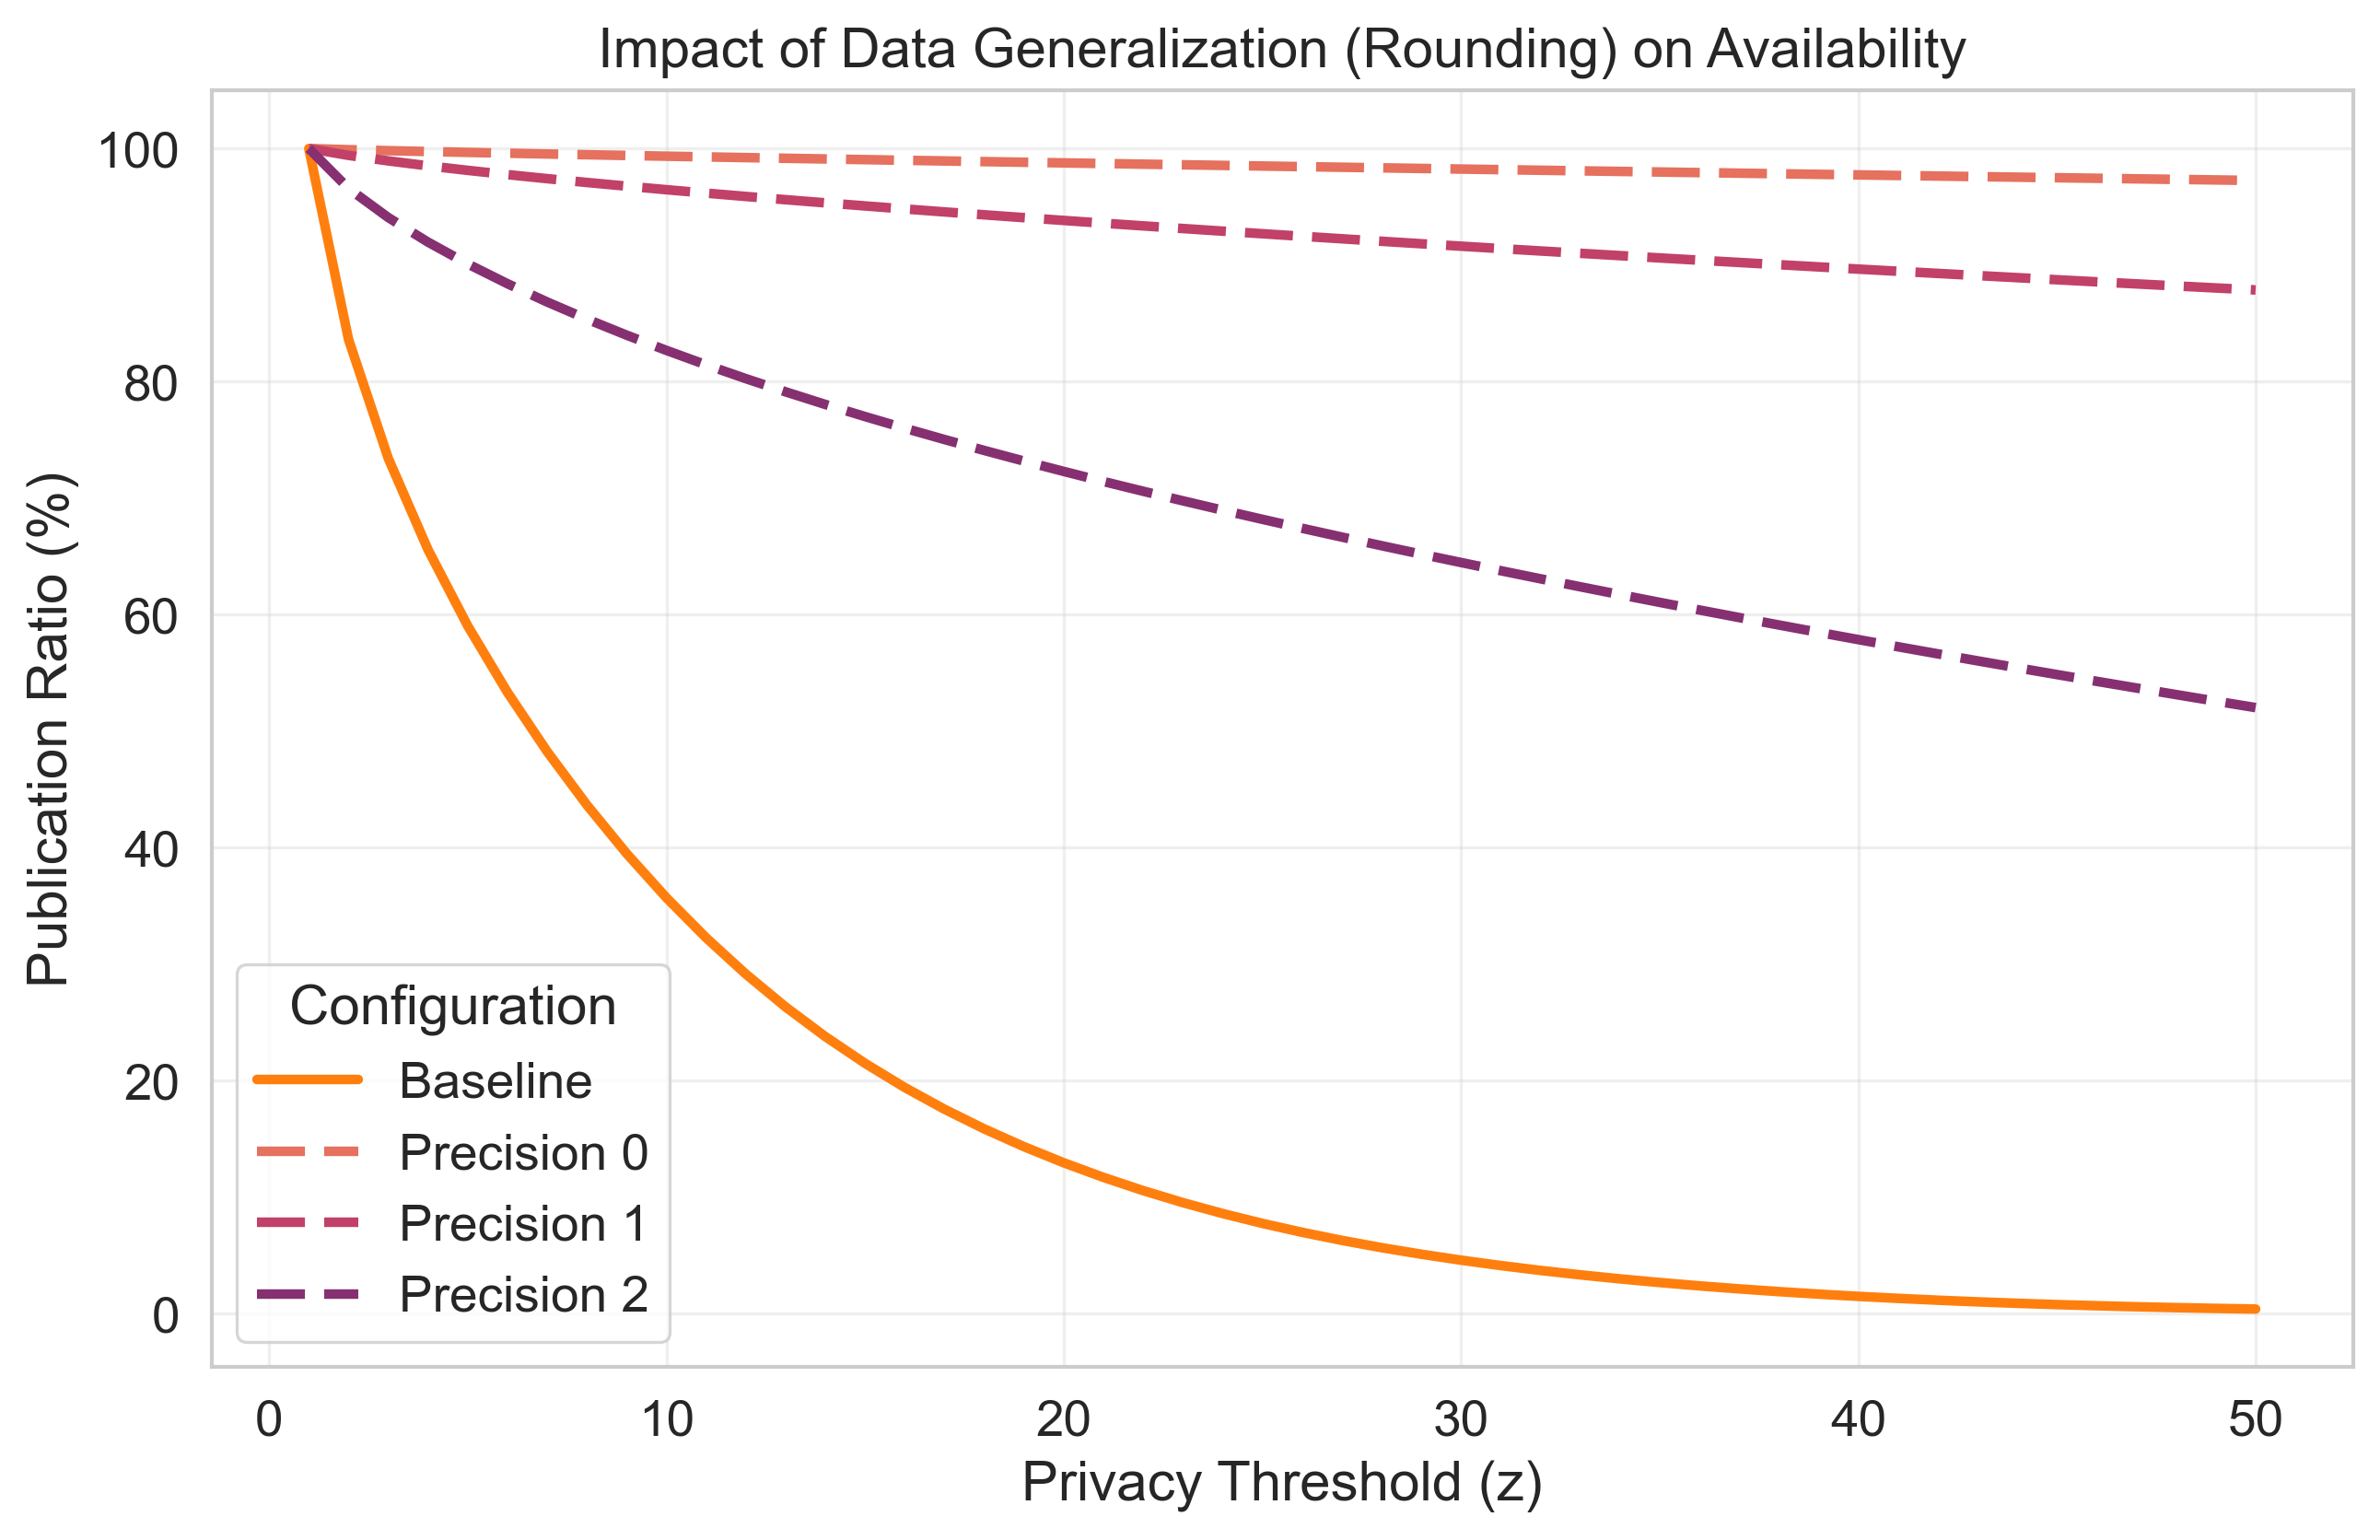
\includegraphics[width=0.8\textwidth]{figures/results_generalization_ratio.png}
\caption{Impact of Data Generalization on Publication Ratio. Lower precision leads to significantly higher data availability.}
\label{fig:results_gen_ratio}
\end{figure}




While reducing precision successfully prevents data suppression, it introduces a permanent loss of information. This cost is first quantified using the $\text{NCP}_{\text{std}}$ metric~\cite{UtilityBasedAnonymizationNCP}, which normalizes the rounding error against the global data range [0, 9.26 kWh].

\begin{figure}[t]
\centering
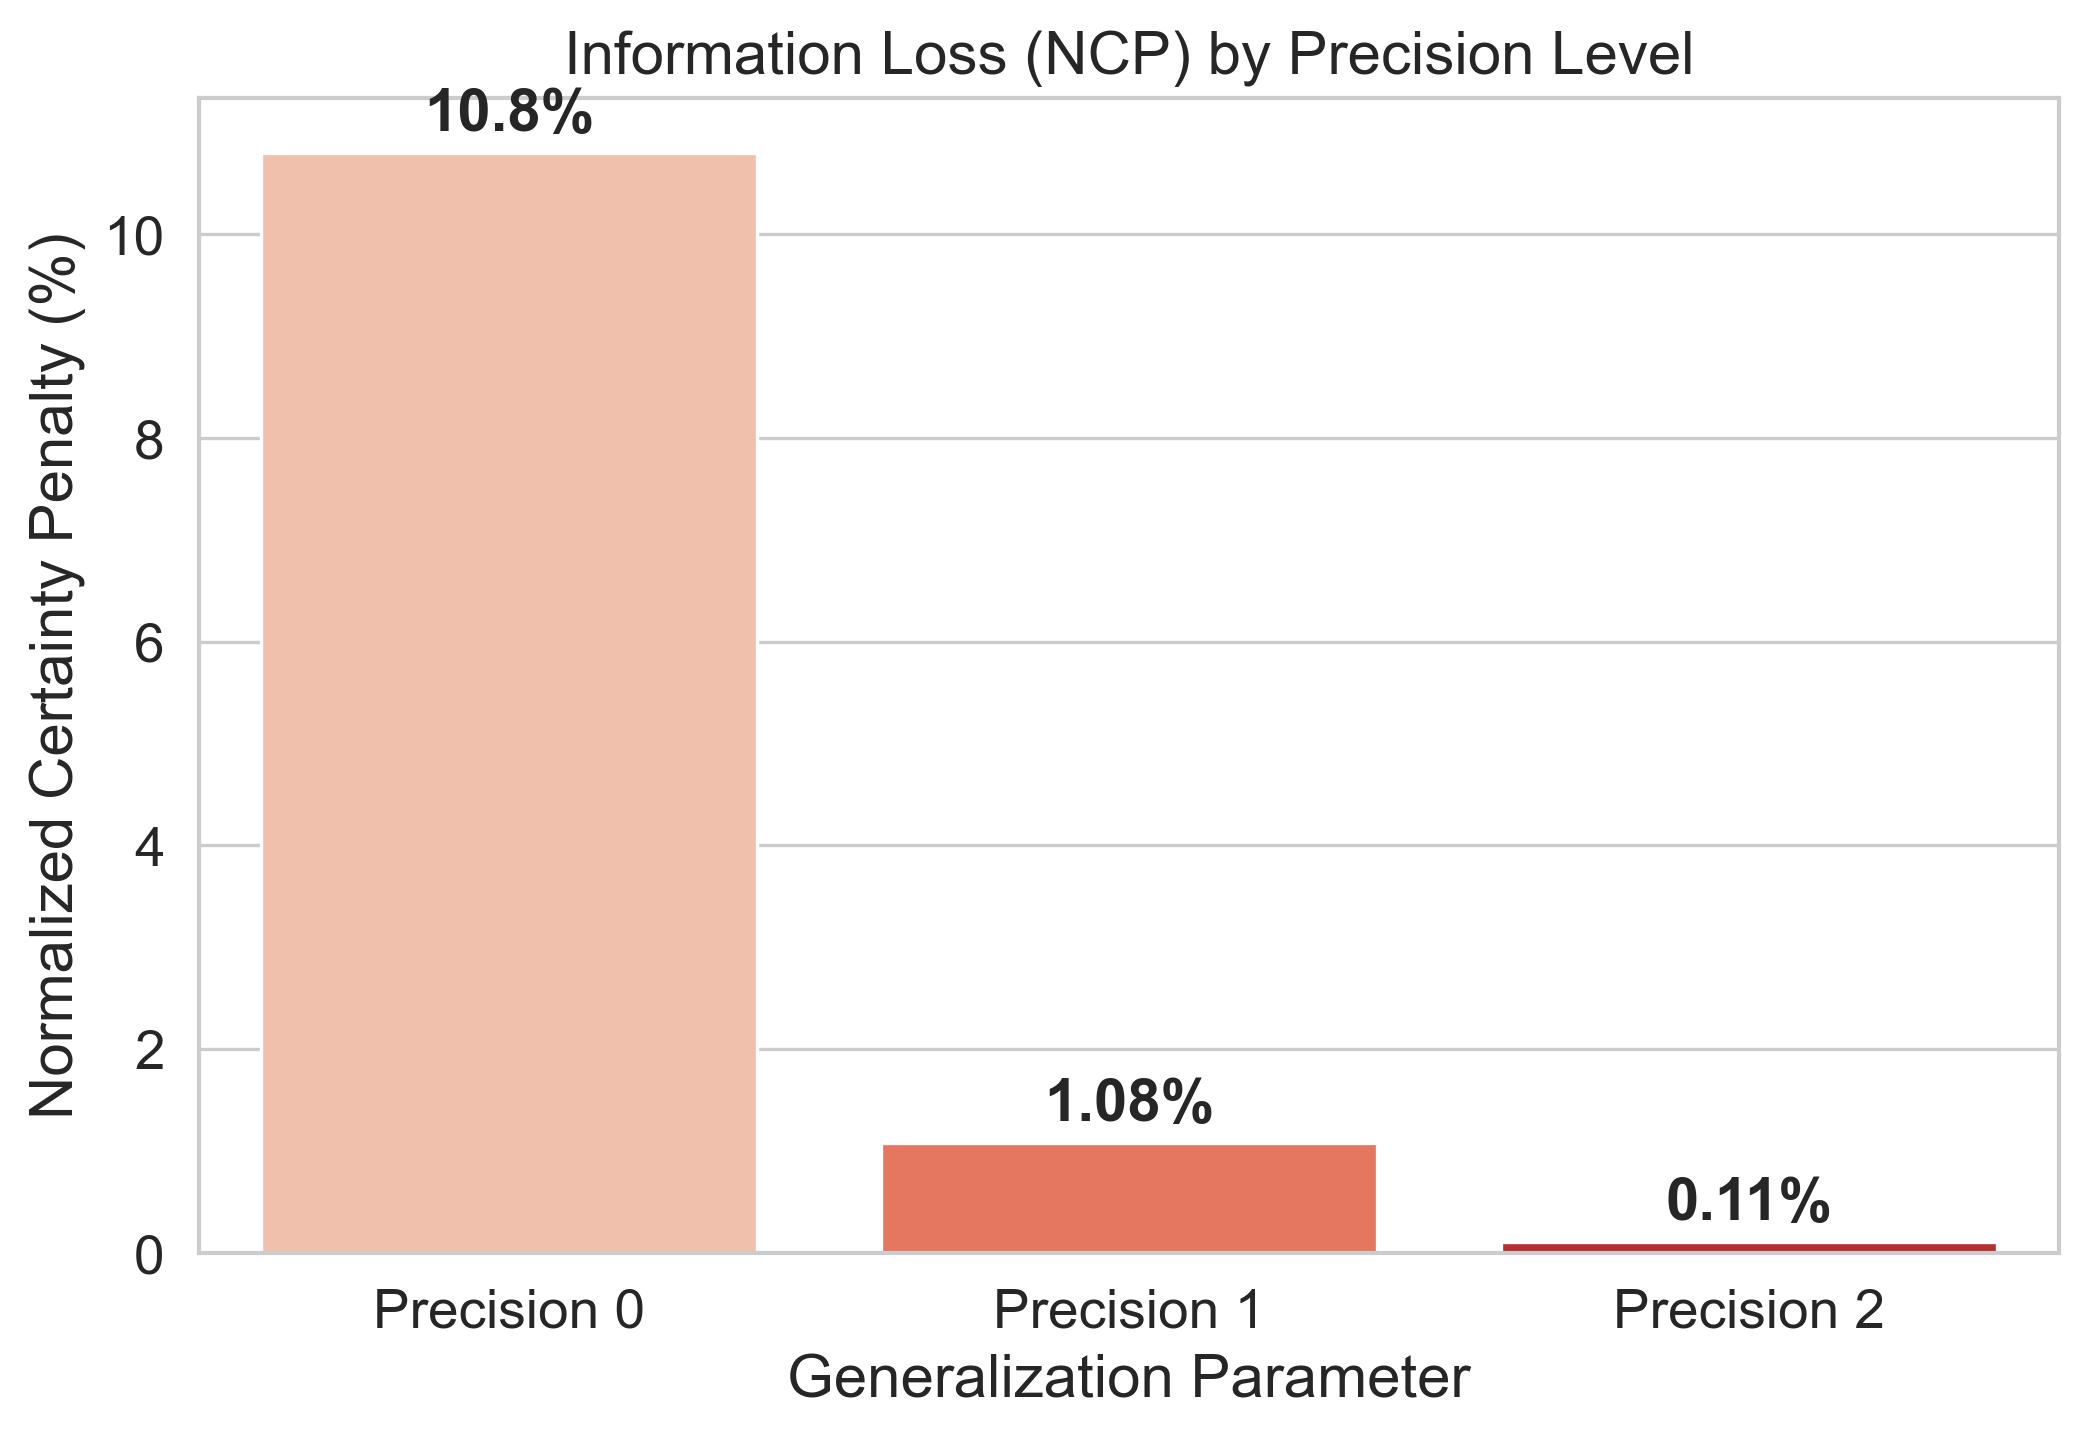
\includegraphics[width=0.77\textwidth]{figures/results_generalization_ncp.png}
\caption{Standard Normalized Certainty Penalty (NCP) for each precision level. The low values suggest a high preservation of global utility.}
\label{fig:results_ncp_std}
\end{figure}

As shown in Figure \ref{fig:results_ncp_std}, the $\text{NCP}_{\text{std}}$ indicates a loss of only 10.8\% for Precision 0 and a negligible 1.1\% for Precision 1. However, these results are skewed by the wide global range caused by outliers, which masks the actual impact of rounding on typical households. To provide a more critical assessment of the utility remaining for the typical user, we contrast these results with the ($\text{NCP}_{\text{eff}}$) defined in Section~\ref{sec:evaluation_metrics}.

\begin{figure}[H]
\centering
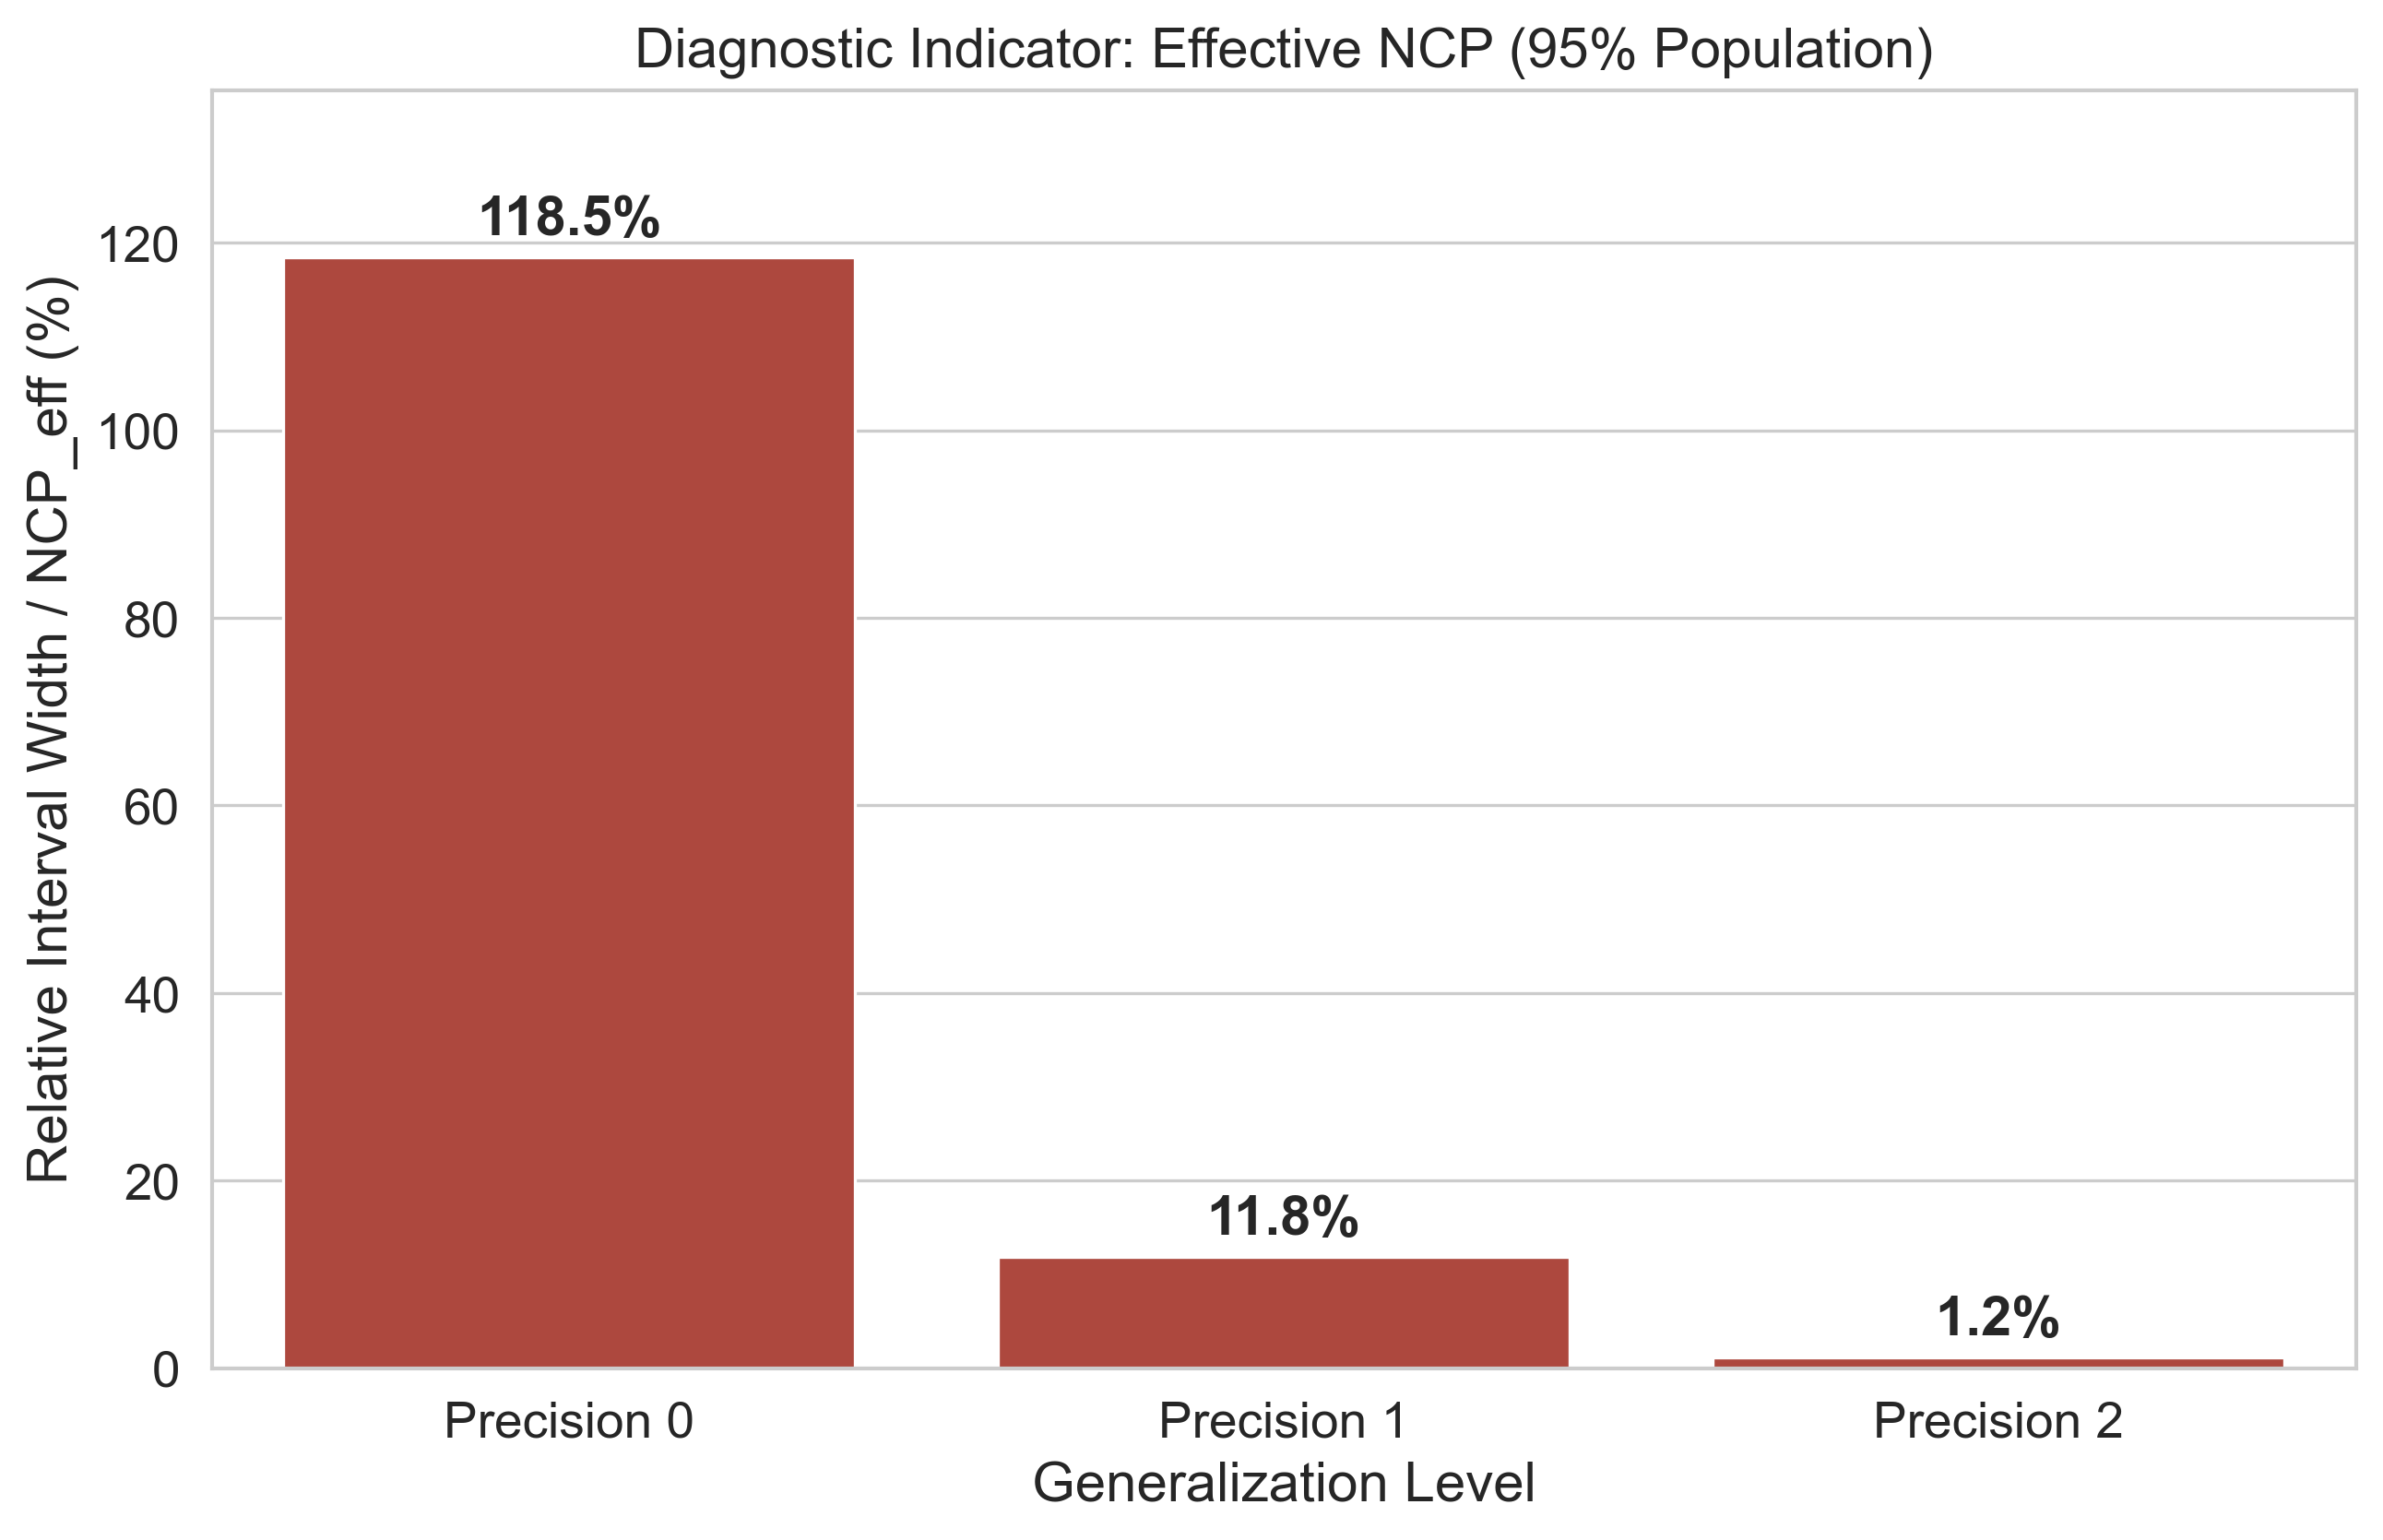
\includegraphics[width=0.75\textwidth]{figures/results_ncp_eff.png}
\caption{Comparison of Standard and Effective NCP. The Effective NCP reveals the true damage to utility for the typical user population.}
\label{fig:encp_comparison}
\end{figure}

The contrast in Figure \ref{fig:encp_comparison} illustrates a significant divergence between the two metrics. While the $\text{NCP}_{\text{std}}$ for Precision 0 is recorded at 10.8\%, the $\text{NCP}_{\text{eff}}$ reaches \textbf{118.5\%}. As defined in the methodology, this value occurs because the rounding interval (1.0 kWh) is numerically larger than the entire consumption span of the 95\% population subset, which covers the interval [0, 0.844 kWh]. In comparison, Precision 1 and Precision 2 yield $\text{NCP}_{\text{eff}}$ values of 11.8\% and 1.2\% respectively, indicating a much closer alignment between the generalization interval and the actual data variance.


% \clearpage


\section{Impact of Temporal Aggregation (Edge)}

The third experimental scenario evaluates the reduction of temporal resolution at the Edge Layer to optimize network performance. Unlike Data Generalization, which modifies numerical values to facilitate grouping, Temporal Aggregation reduces the frequency of data transmission by representing multiple 30-minute intervals with a single arithmetic mean.

Figure \ref{fig:results_agg_bw} illustrates the Bandwidth Savings achieved across the three tested window sizes ($W \in \{1\,\text{h}, 2\,\text{h}, 4\,\text{h}\}$).

\begin{figure}[H]
\centering
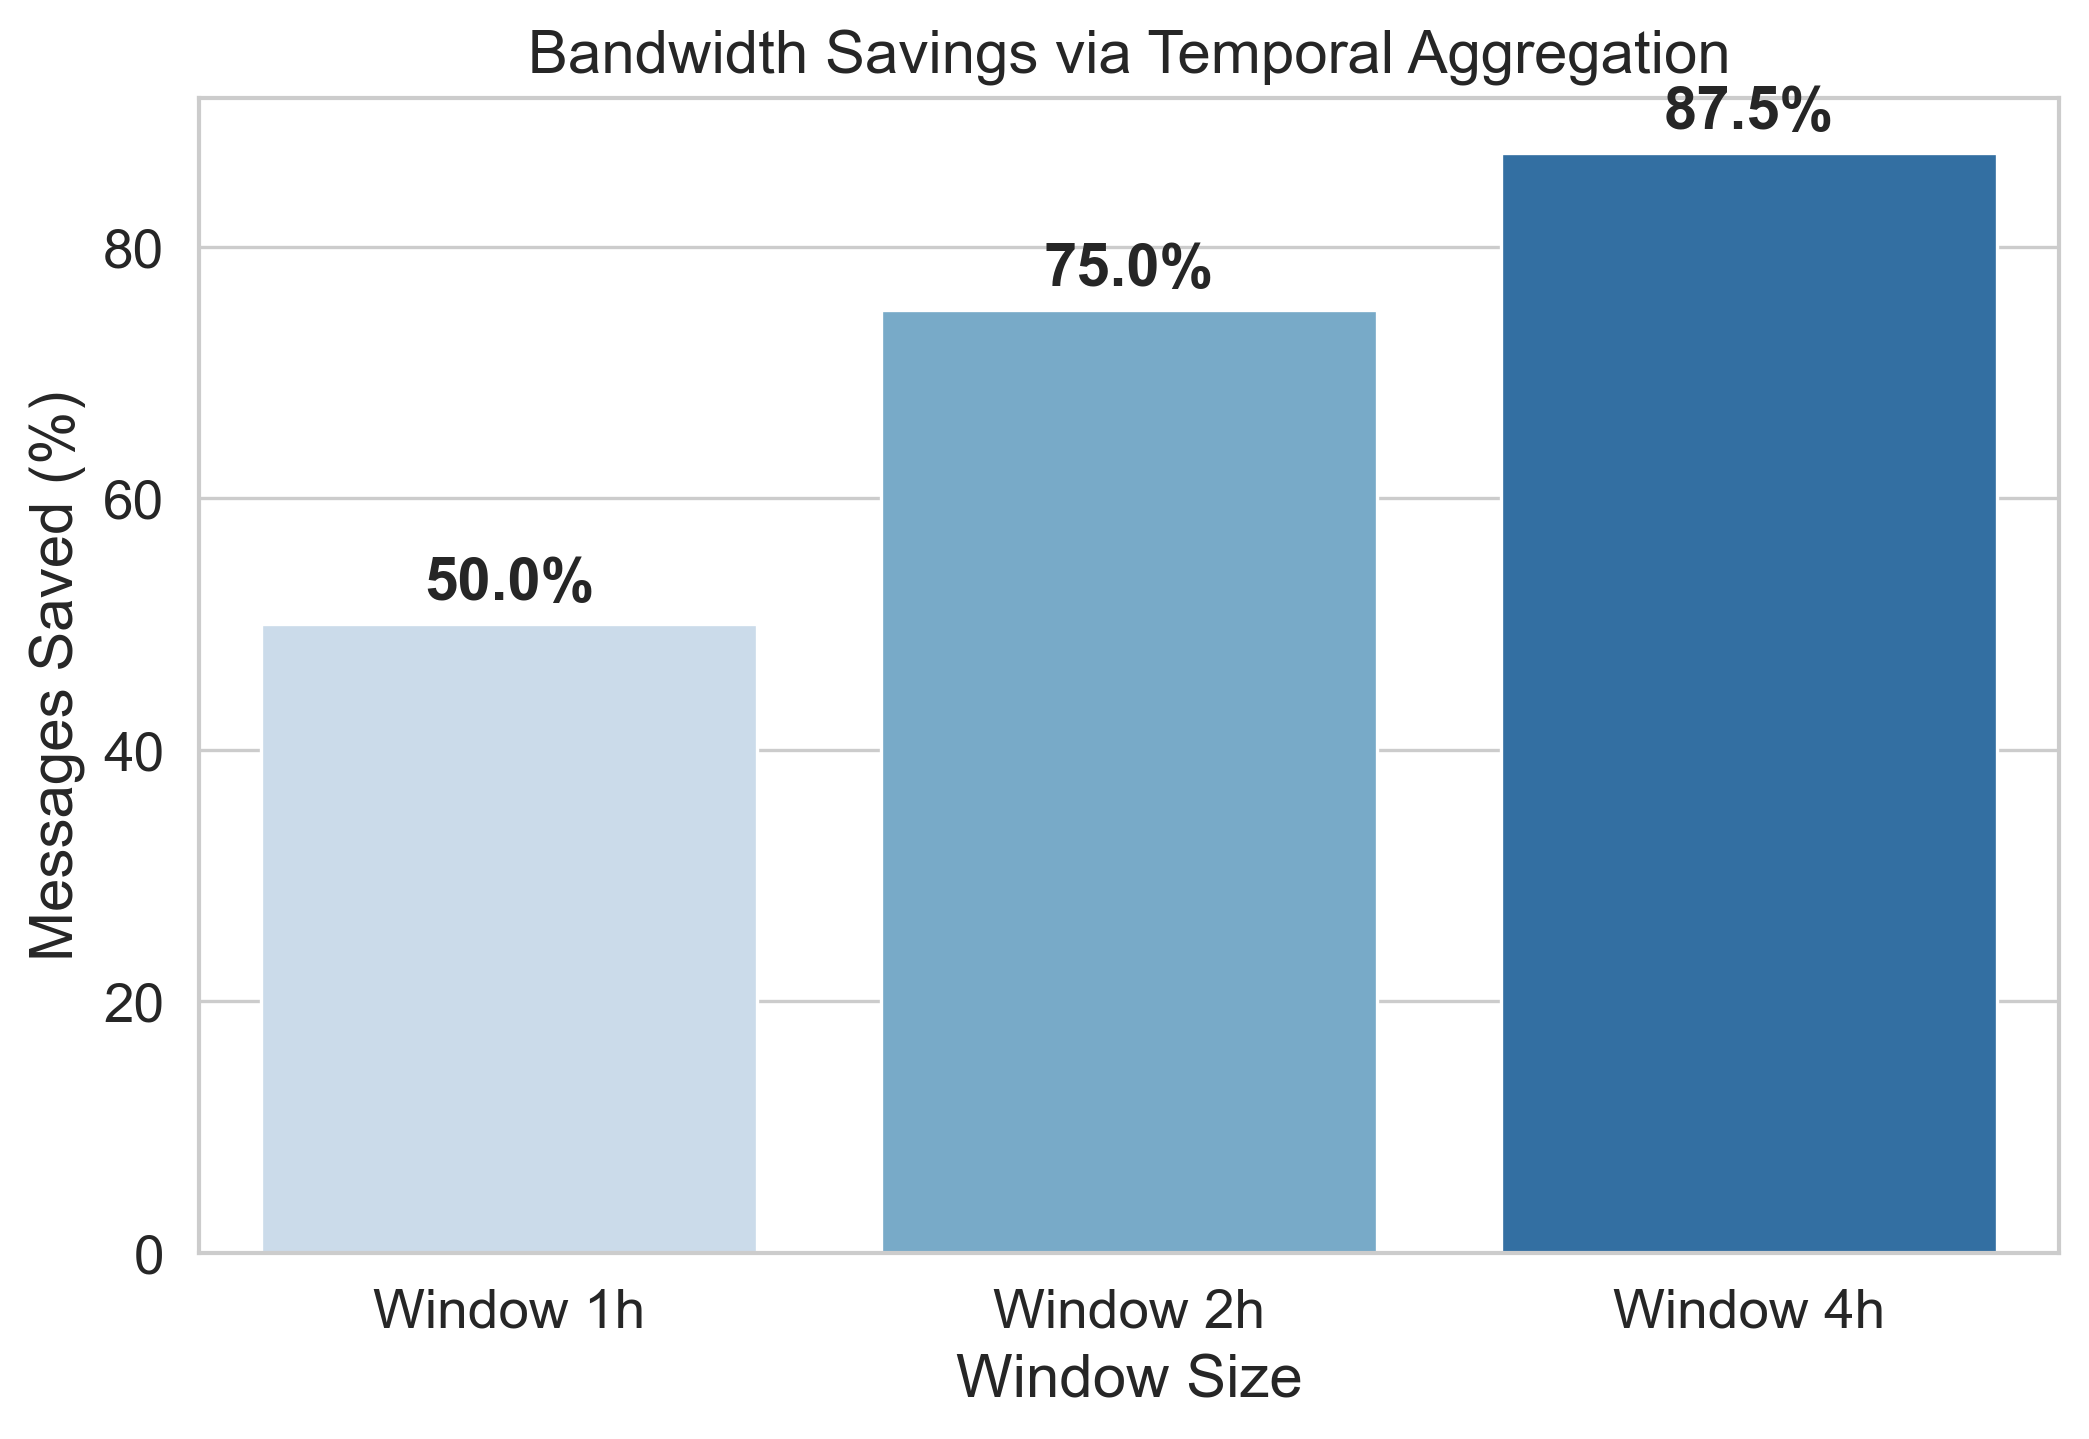
\includegraphics[width=0.75\textwidth]{figures/results_aggregation_bandwidth.png}
\caption{Bandwidth Savings achieved through non-overlapping (tumbling) time windows joining $n$ timestamps. Savings increase with the window size, following a $1-1/n$ relationship.}
\label{fig:results_agg_bw}
\end{figure}


The results confirm that bandwidth savings follow a deterministic relationship ($1-1/n$), where $n$ represents the number of original 30-minute timestamps consolidated into each window. For instance, the 2h window joins $n=4$ intervals, resulting in the theoretical $1 - 1/4 = 75\%$ savings observed in the data.

\begin{itemize}
    \item \textbf{Window 1h (n=2):} Results in a 50.0\% reduction in transmitted tuples, as two 30-minute readings are consolidated into one.
    \item \textbf{Window 2h (n=4):} Achieves 75.0\% savings, significantly reducing the communication overhead for the Edge nodes.
    \item \textbf{Window 4h (n=8)}: Provides the highest performance gain of 87.5\% among the tested configurations, representing an 8-to-1 reduction in data volume.
\end{itemize}

These results show that temporal aggregation enables a predictable reduction in data volume, reaching 87.5\% for the 4h window, while the corresponding Publication Ratio follows the 30-minute baseline trend with minimal deviation.

To assess the impact of these performance gains on data utility, Figure \ref{fig:results_agg_privacy} compares the global publication ratio of the aggregated windows against the 30-minute baseline.

\begin{figure}[H]
\centering
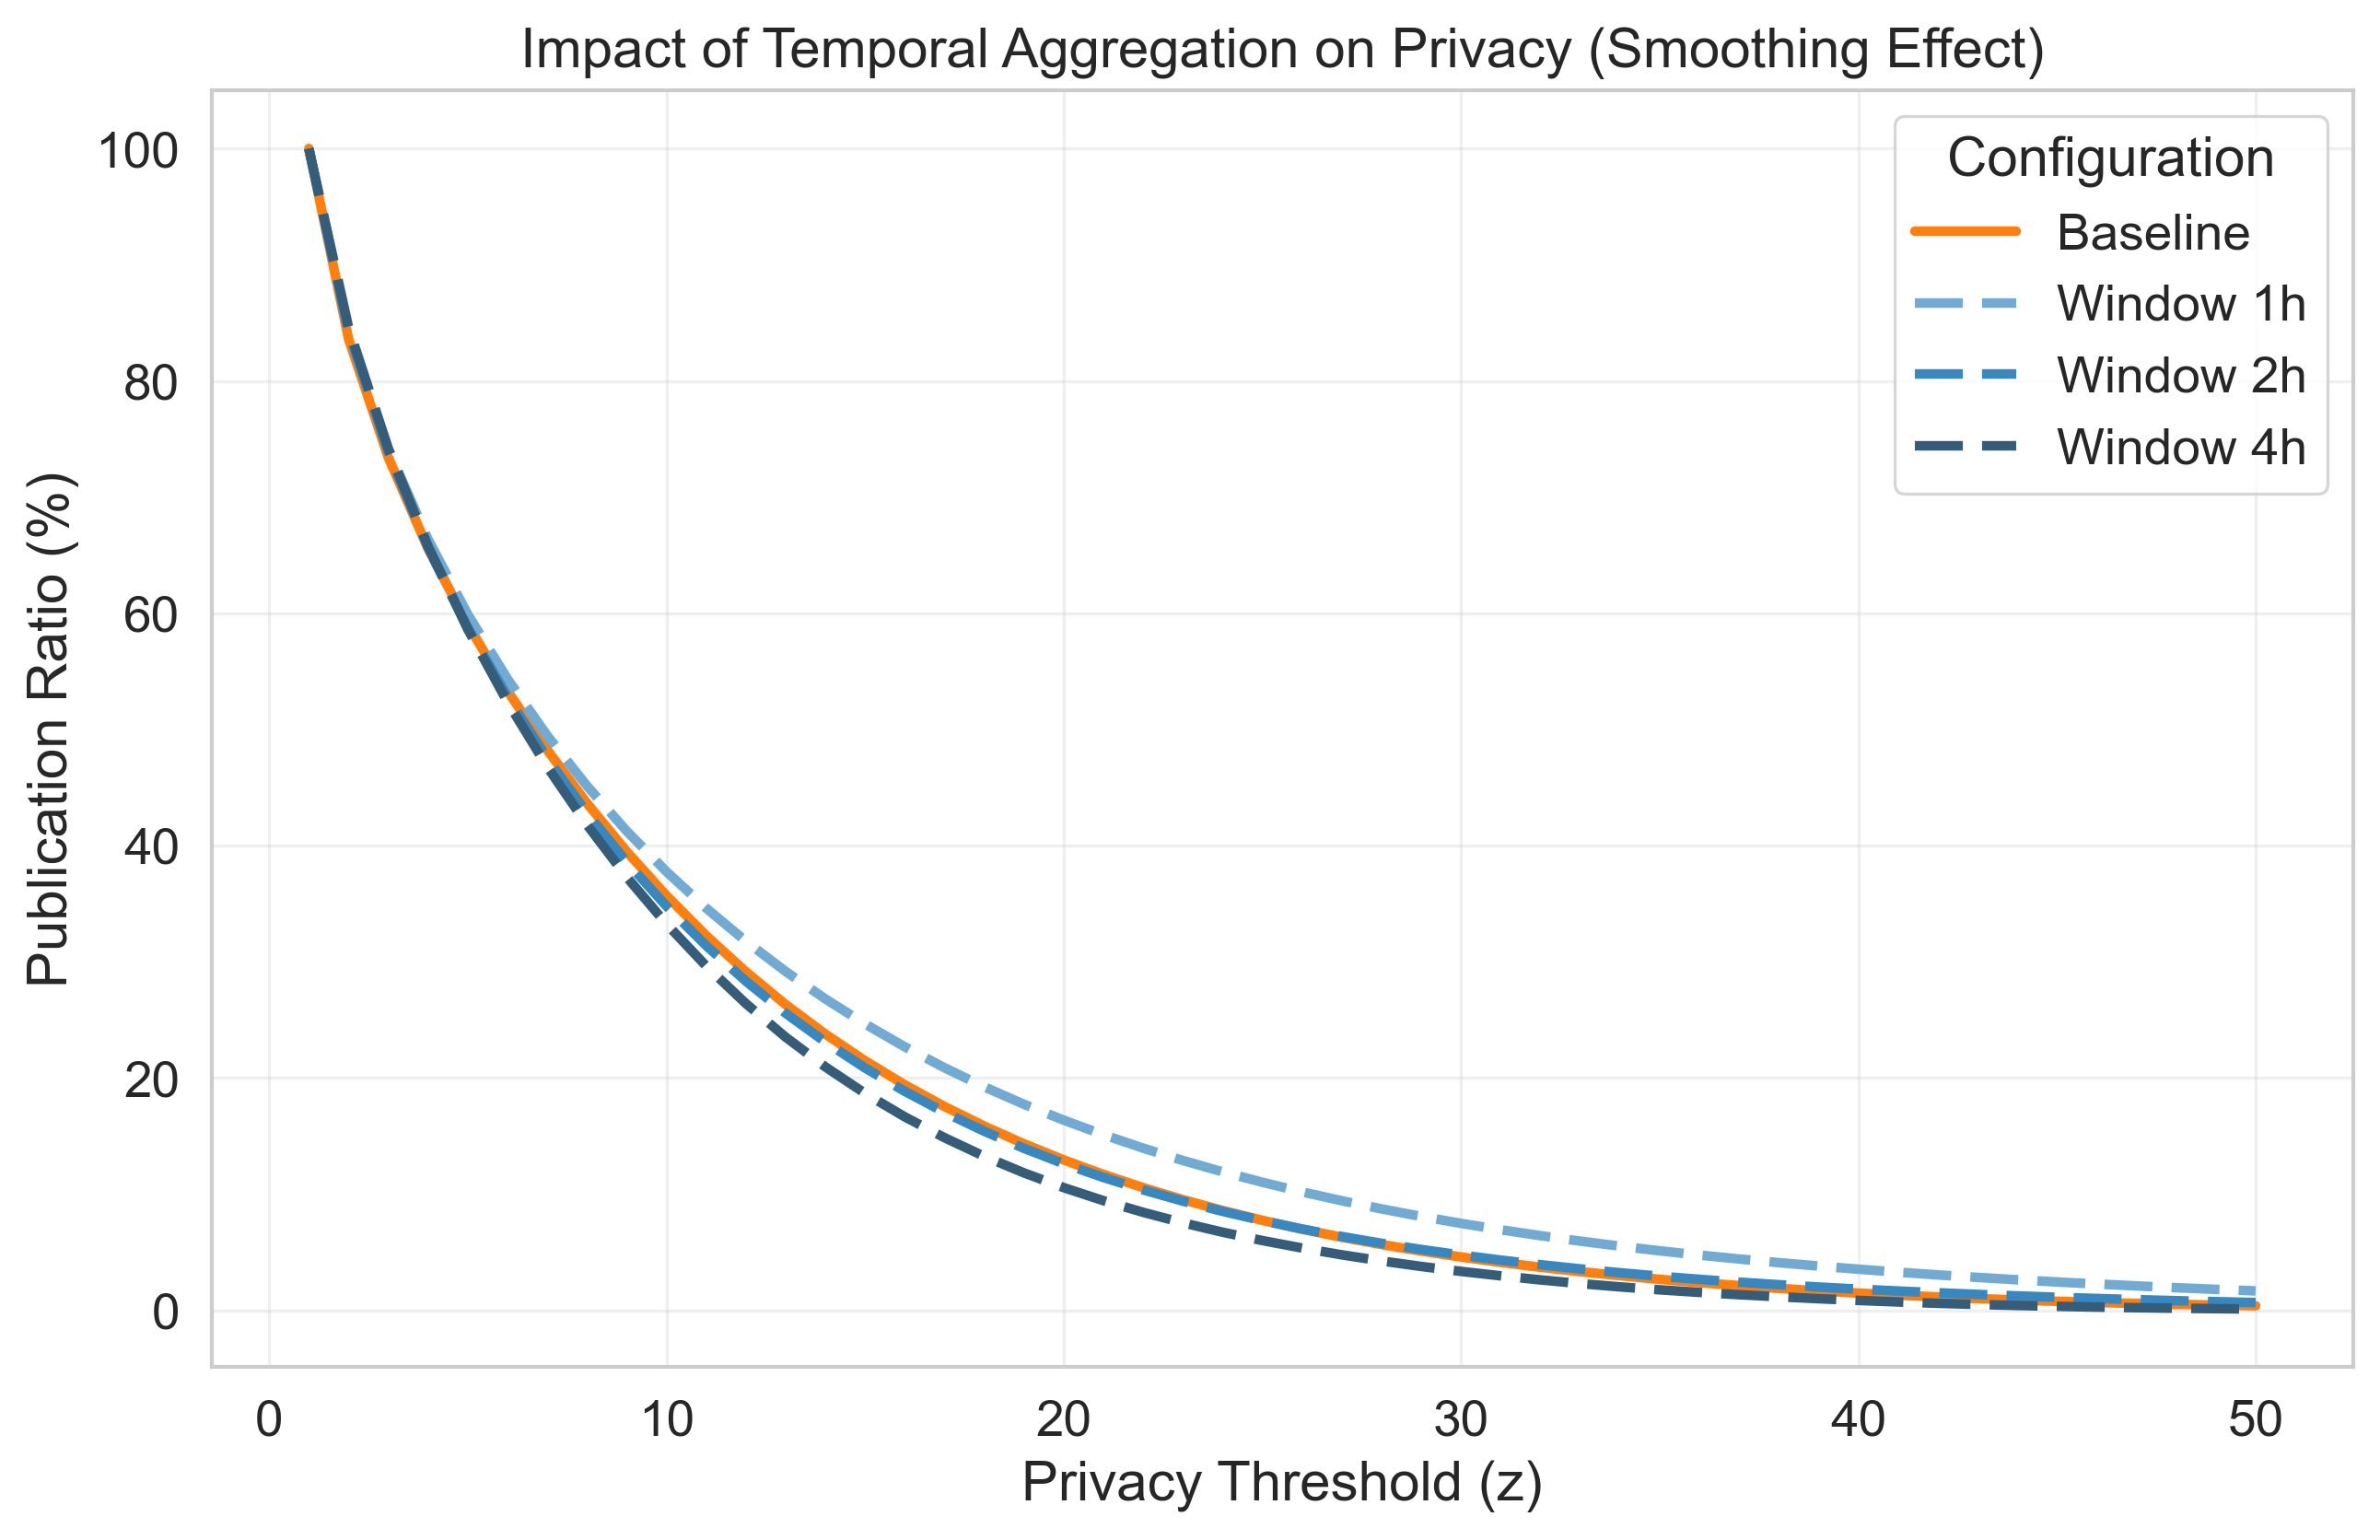
\includegraphics[width=0.85\textwidth]{figures/results_aggregation_privacy.png}
\caption{Comparison of Publication Ratio: Baseline vs. Aggregated Windows. Aggregation results maintain near-total parity with the baseline across all tested thresholds.}
\label{fig:results_agg_privacy}
\end{figure}




The experimental data illustrated in Figure \ref{fig:results_agg_privacy} shows that the publication ratios for the aggregated windows follow a trajectory nearly identical to the 30-minute baseline. Across the tested range of $z$, the availability for the \textbf{Window 1h} and \textbf{Window 2h} scenarios remains marginally higher than the baseline. Specifically, at the highest tested threshold of $z=50$, the 1h window reports a publication ratio of 1.68\%, compared to the 0.40\% observed in the baseline.

The \textbf{Window 4h} scenario results in an 87.5\% reduction in total record count. At $z=50$, its publication ratio (0.11\%) remains within a 0.3 percentage point absolute range of the baseline. Across all tested configurations, the difference in data availability between the 30-minute raw data and the aggregated windows does not exceed a 1.3 percentage point absolute margin at $z=50$.


\section{Impact of Local Prefiltering}
\label{sec:localprefiltering}

The final scenario evaluates a distributed architecture where the privacy-preserving workload is shared between the Fog gateways and the Central Entity. This hybrid approach combines data generalization at the Edge with a Snapshot $z$-anonymity check at the Fog Layer. For this configuration, a fixed precision of \textbf{$p=2$ decimal places} was chosen. As justified in the methodology (Section~\ref{sec:scenarios}), this choice was based on a preliminary analysis which revealed that raw data ($p=3$) is too unique within a small 100-user neighborhood to satisfy a local $z$-threshold, leading to near-total suppression at the gateway. Generalizing to two decimal places provides the minimum data density required to make localized prefiltering a viable architectural strategy.


% This hybrid approach combines data generalization ($p=2$) at the Edge with a snapshot $z$-anonymity check at the Fog level.


Figure \ref{fig:results_prefilter_ratio} illustrates the global publication ratio for three local thresholds ($z_{\text{local}} \in \{2, 5, 10\}$) compared to the raw 30-minute baseline. To establish an upper bound for data utility, a standalone $p=2$ generalization curve (Edge Only) is included as a reference.

\begin{figure}[H]
\centering
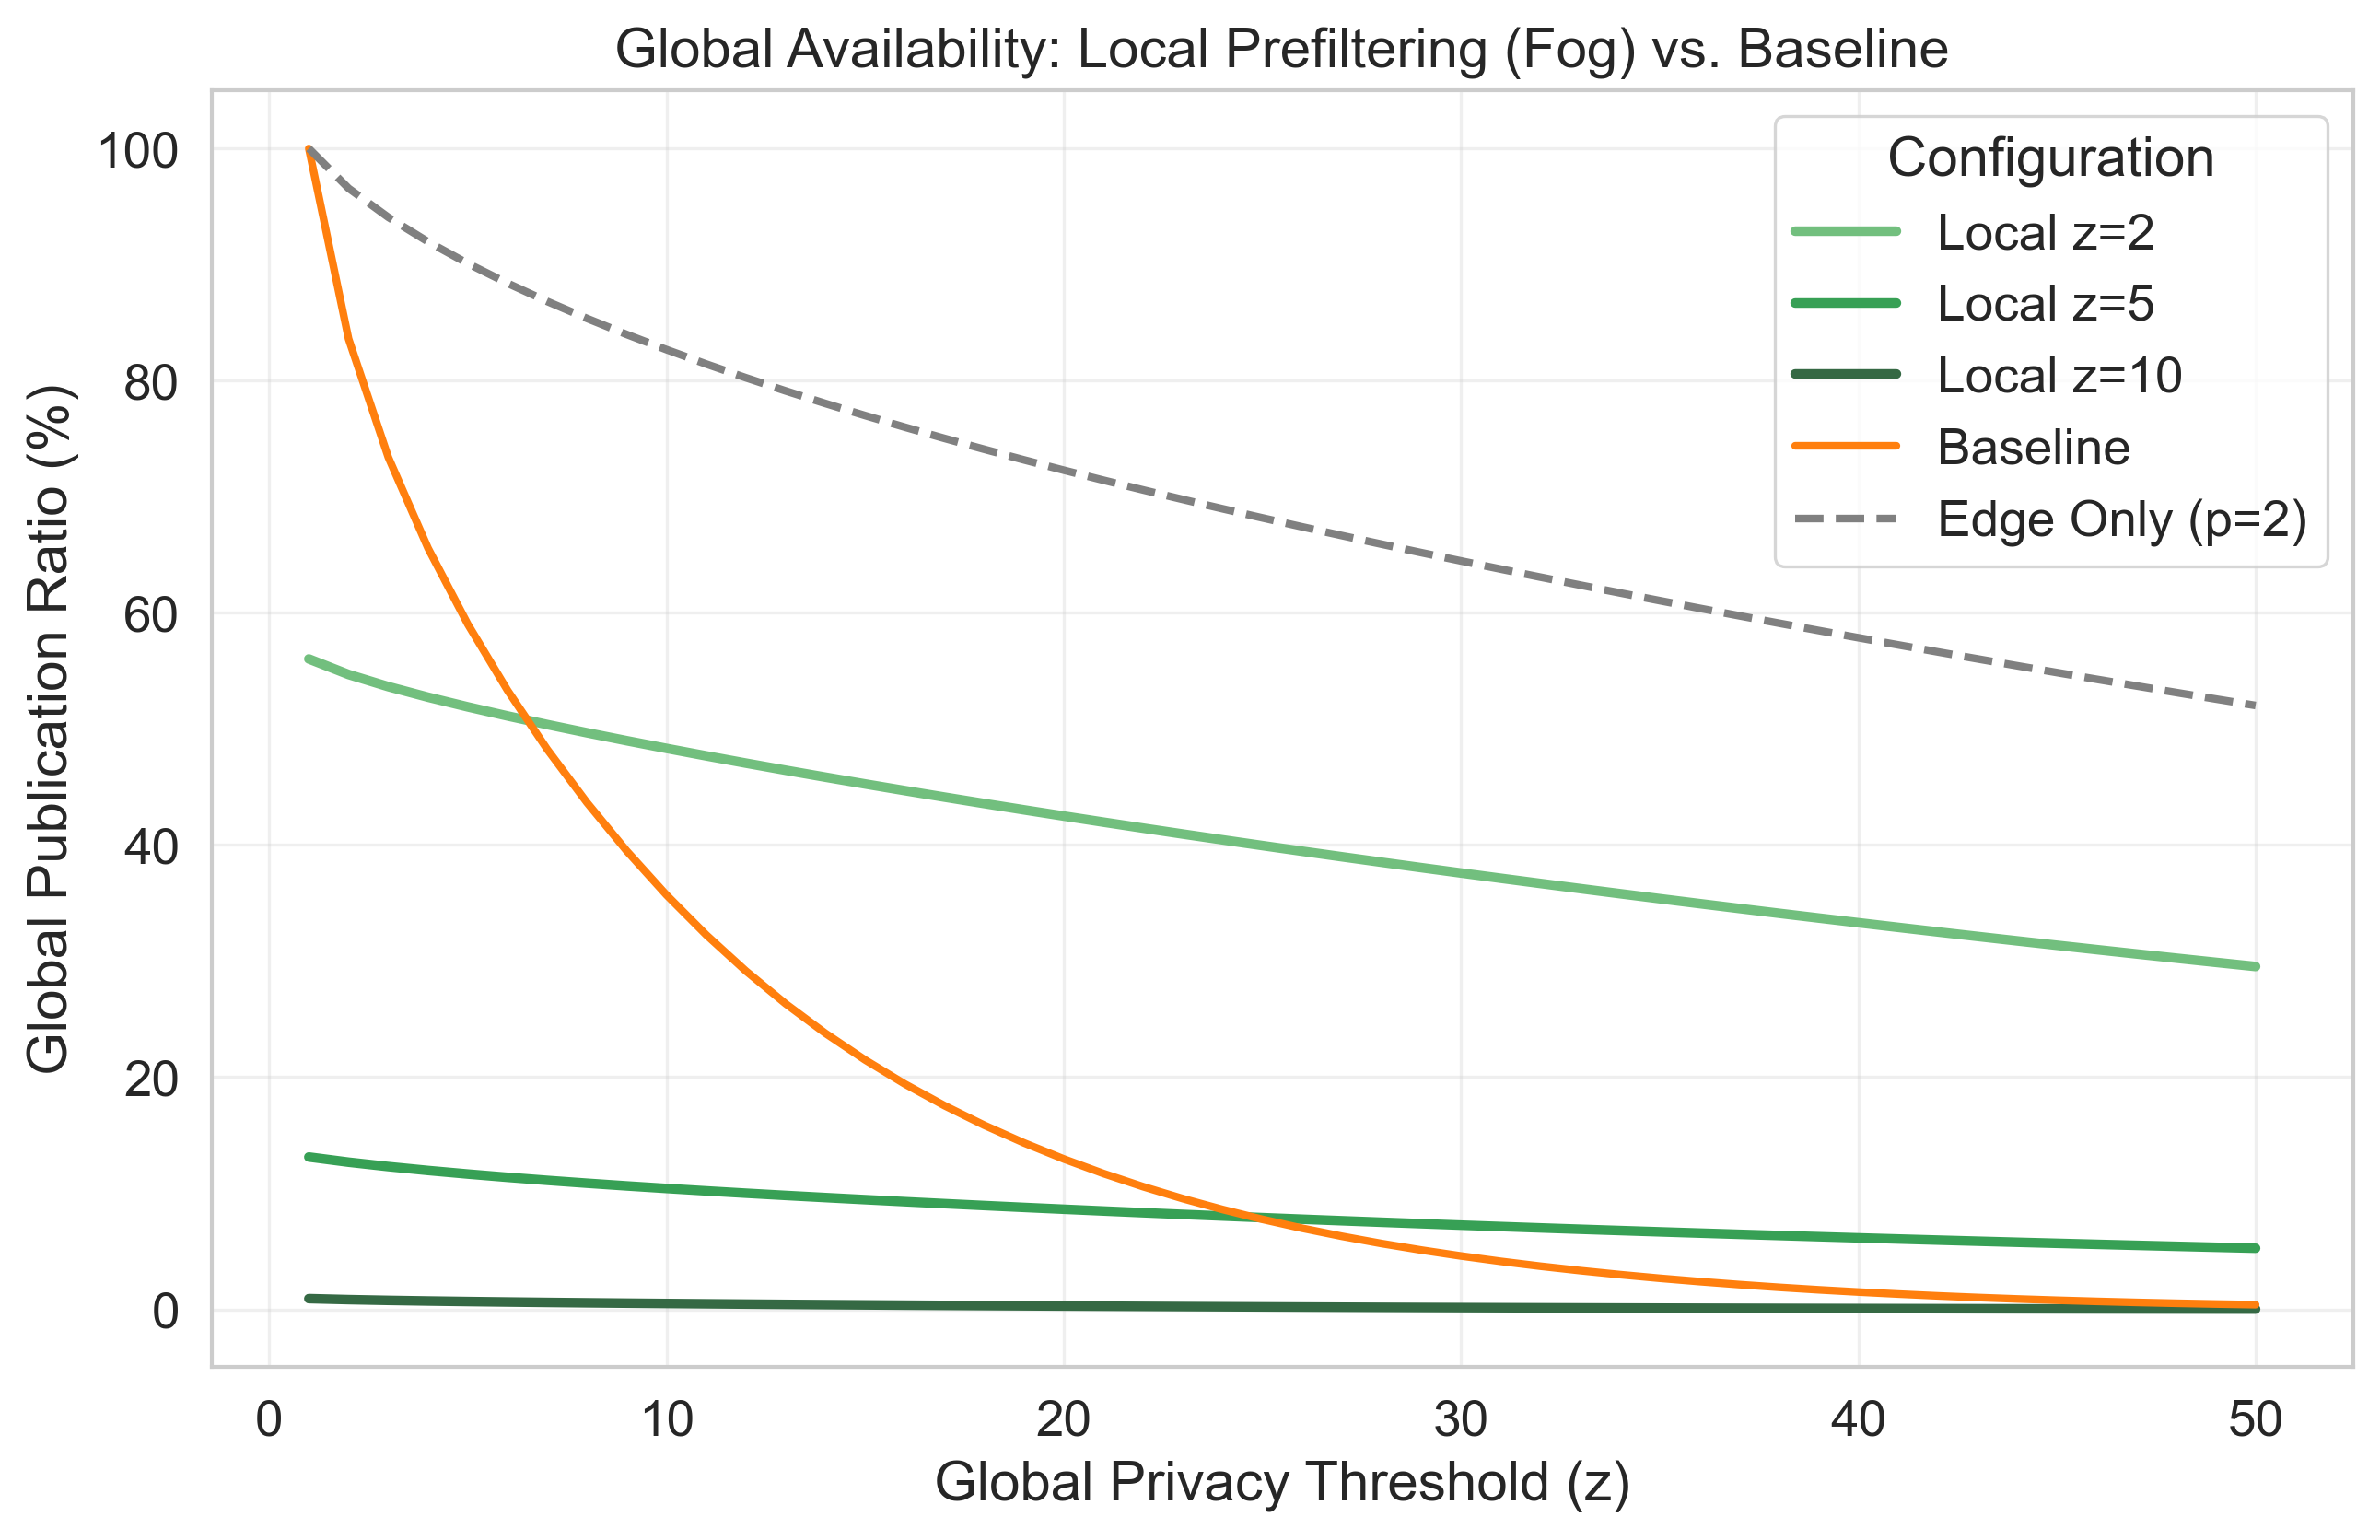
\includegraphics[width=0.85\textwidth]{figures/results_prefiltering_ratio.png}
\caption{Global Publication Ratio after Local Prefiltering. Availability is heavily dependent on the local suppression threshold.}
\label{fig:results_prefilter_ratio}
\end{figure}


The data reveals two distinct behaviors driven by the interaction between precision reduction and local filtering:

\begin{itemize}
    \item \textbf{Initial Suppression:} At $z=1$, the \textbf{Local $z=2$} scenario publishes 56.03\% of data, representing a 43.97 percentage point absolute drop compared to the 100\% availability of the standalone Edge Only $p=2$ reference. Because both scenarios use identical Edge rounding, this initial gap represents the suppression overhead introduced by the Fog Layer. Data that is frequent enough globally is suppressed because it fails to meet the threshold within its specific local neighborhood. The \textbf{Local $z=5$} and \textbf{Local $z=10$} scenarios experience even steeper initial suppression, starting at 13.12\% and 0.92\% respectively.
    \item \textbf{Decline Rate:} Despite the lower starting points, the prefiltering curves follow a slow-decay trajectory nearly parallel to the standalone Edge Only $p=2$ reference, rather than the sharp drop of the raw baseline. At $z=50$, the raw baseline falls to 0.4\%, whereas the \textbf{Local $z=2$} scenario maintains 29.53\% availability (compared to 52.02\% for the standalone $p=2$ case). The absolute gap between these two curves narrows as $z$ increases, shifting from a 43.98 percentage point difference at $z=1$ to 22.49 percentage points at $z=50$.
\end{itemize} 

Figure \ref{fig:results_prefilter_offloading} illustrates the "Success Rate at Cloud", which measures the percentage of tuples that were not suppressed by the local Fog Layer filter and subsequently satisfied the global $z$ requirement.

\begin{figure}[H]
\centering
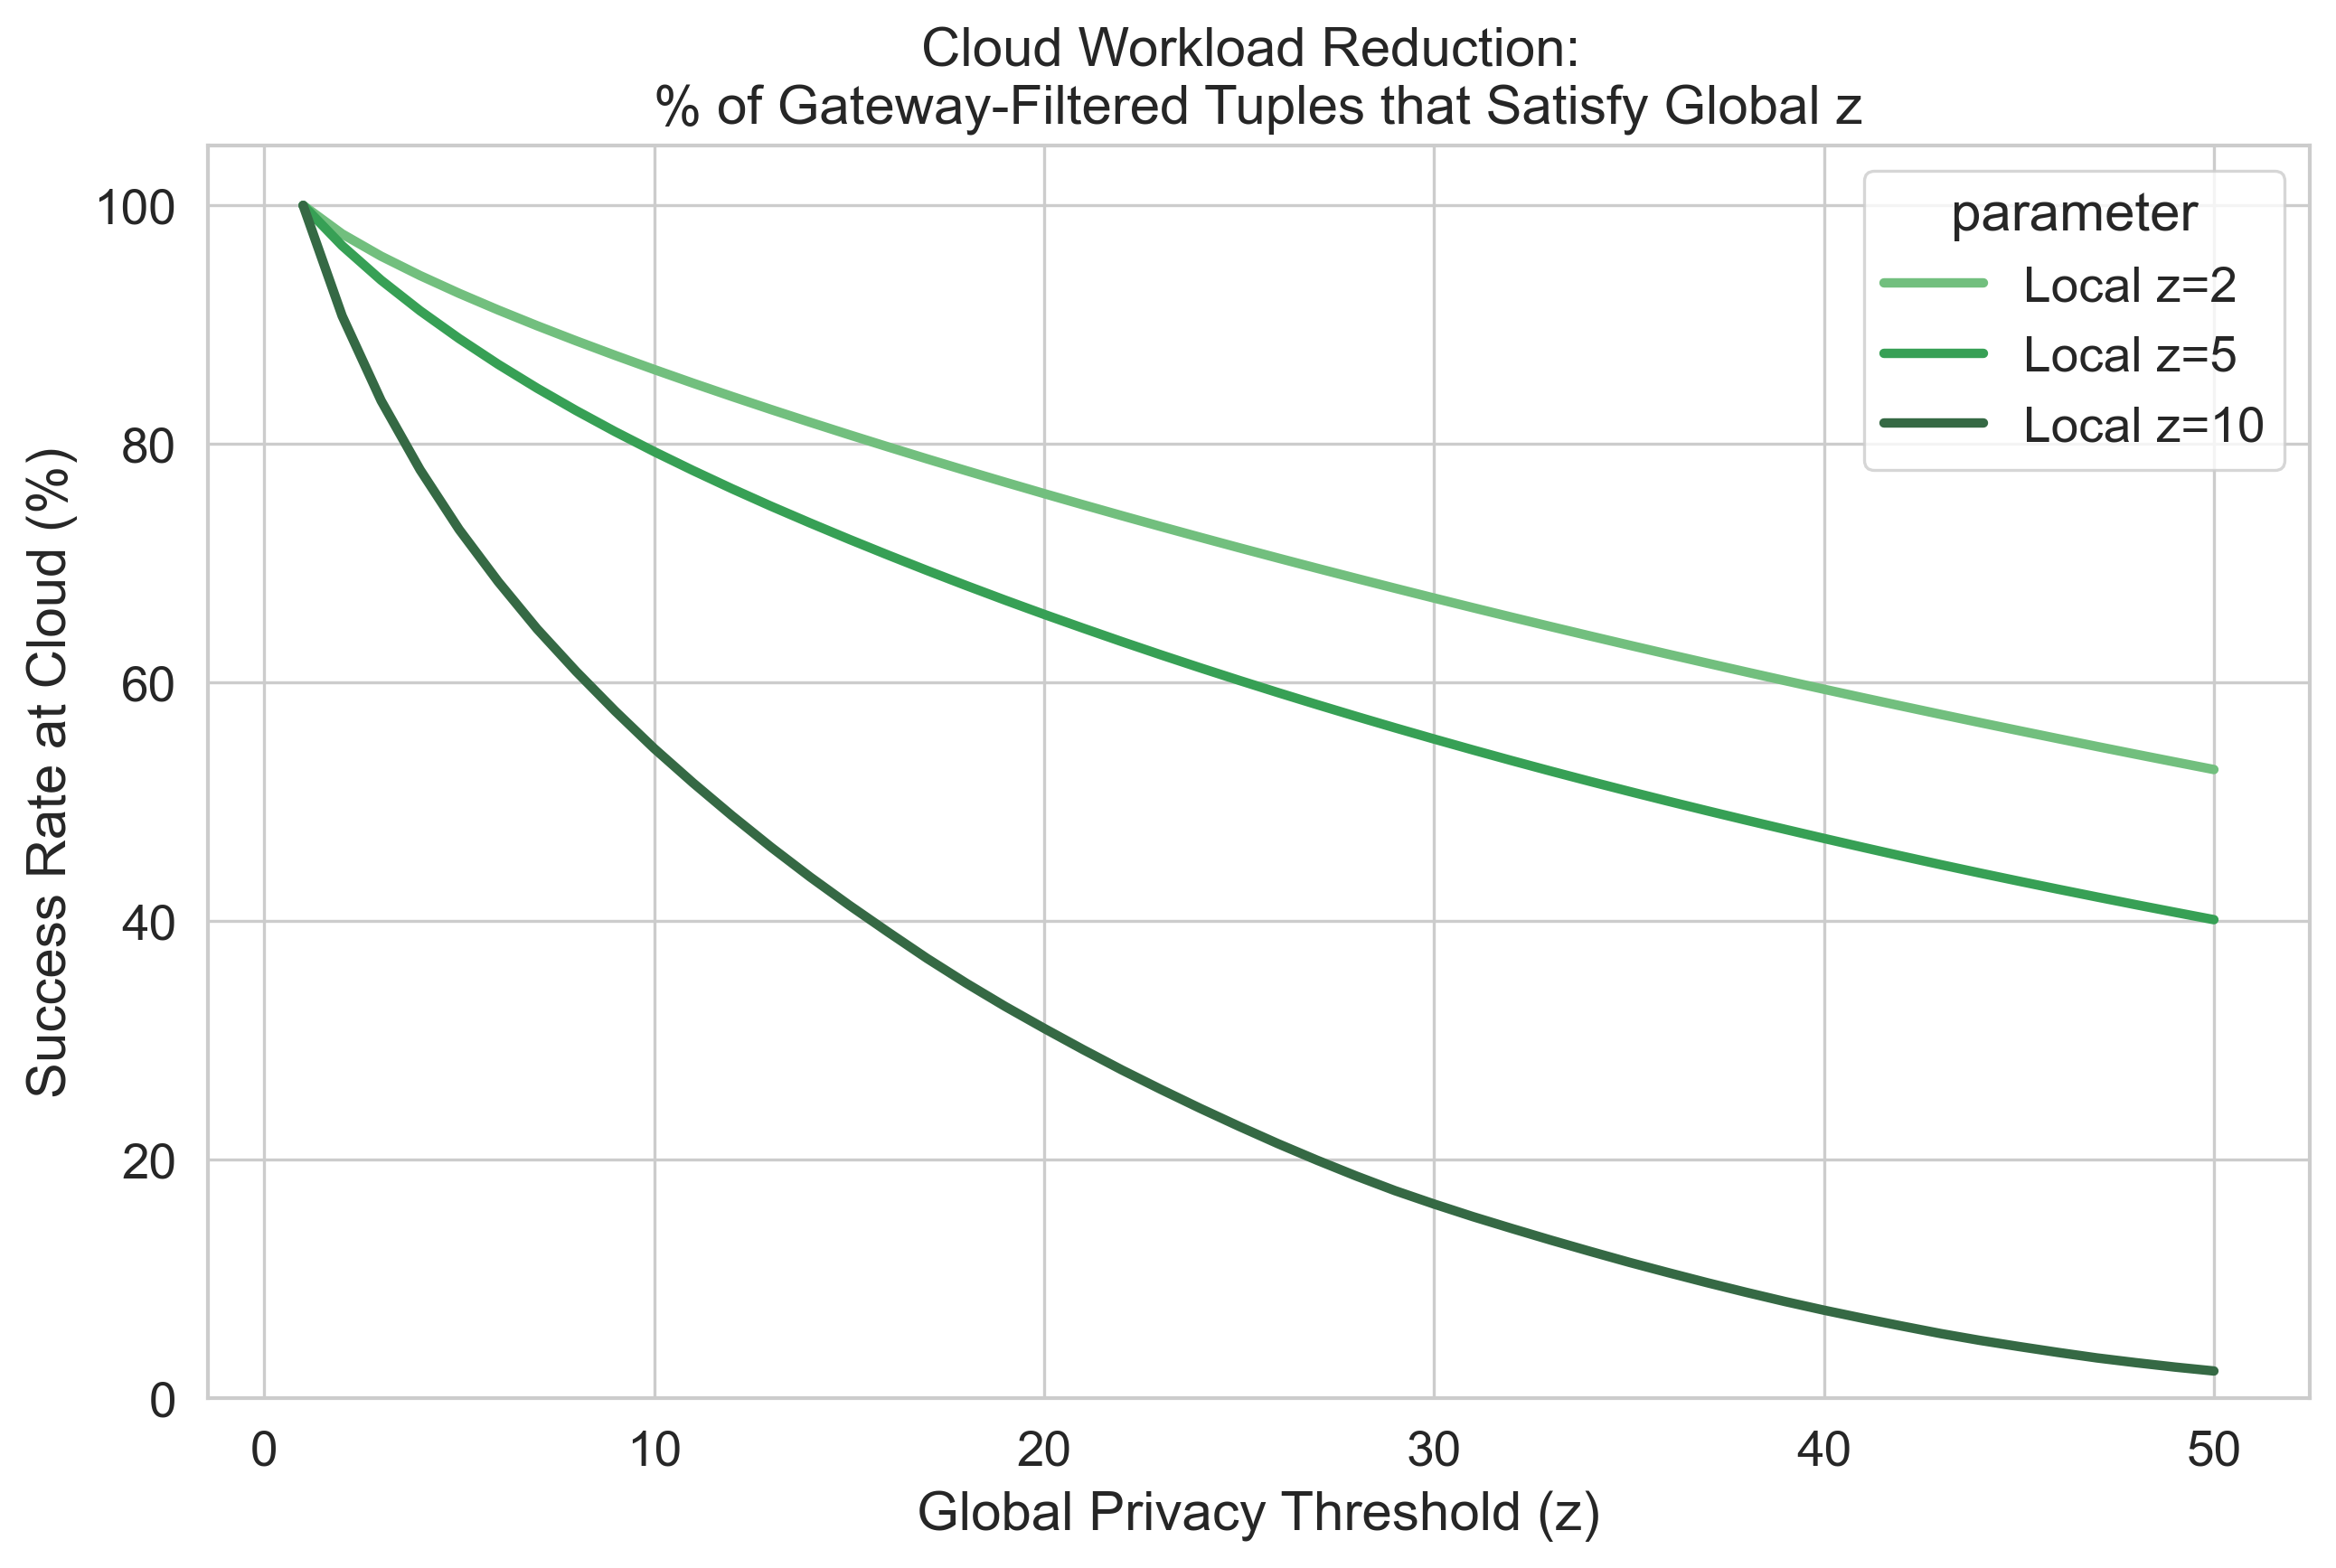
\includegraphics[width=0.85\textwidth]{figures/results_prefiltering_offloading.png}
\caption{Cloud Workload Reduction: Percentage of Gateway-Filtered tuples that satisfy the Global z threshold.}
\label{fig:results_prefilter_offloading}
\end{figure}




The data shows that while all scenarios begin with a 100\% success rate at $z=1$, the proportion of Fog-approved tuples that pass the Cloud-level check decreases as the global threshold $z$ increases. This decline is most pronounced in the \textbf{Local $z=10$} scenario, where the success rate drops to approximately 2.29\% at $z=50$. This trend indicates a cumulative suppression effect: because the gateways subtract $(z_{\text{local}} - 1)$ from the local counts before forwarding, the Central Entity receives a significantly reduced data stream. Consequently, this depletion causes the success rate to drop even when the global threshold matches the local filter (e.g., when both are set to $z=5$). Furthermore, this mechanism explains why the success rate falls much faster for $z_{\text{local}}=10$ and $z_{\text{local}}=5$ compared to $z_{\text{local}}=2$. A higher local threshold filters out a significantly larger portion of tuples at the Fog Layer, resulting in a much smaller surplus being forwarded. Consequently, to survive the final global check, multiple gateways must simultaneously report a surplus for the exact same value, which becomes increasingly improbable when the forwarded volumes are already severely depleted by strict local filters.


In addition to the impacts on data utility, this scenario results in a reduction of message volume between the Fog and Cloud Layers. By suppressing unique outliers before they traverse the core network, the architecture generates significant bandwidth savings. Because a global threshold of $z=1$ effectively disables suppression at the Central Entity (as any count $\geq 1$ is published), the global publication ratio at this point strictly reflects the data that passed the local gateways. Therefore, the data "missing" at $z=1$ in Figure \ref{fig:results_prefilter_ratio} represents the exact percentage of tuples blocked at the Fog Layer, translating directly to the following bandwidth savings:

\begin{itemize}
    \item \textbf{Local $z=2$:} Achieves a 43.97\% reduction in message volume.
    \item \textbf{Local $z=5$:} Achieves an 86.88\% reduction, effectively removing the vast majority of unique consumption spikes from the stream.
    \item \textbf{Local $z=10$:} Suppresses 99.08\% of all generated data at the gateway level.
\end{itemize}

The data shows a consistent inverse relationship between bandwidth savings at the Fog Layer and subsequent data availability at the Central Entity. As the local threshold increases from $z_{\text{local}}=2$ to $z_{\text{local}}=10$, the resulting bandwidth savings increase from 43.97\% to 99.08\%, while the initial global publication ratio ($z=1$) decreases from 56.03\% to 0.92\%. Across the evaluated configurations, the local threshold acts as an upper bound for the maximum achievable data utility at the Central Entity.
\chapter{Discussion}
\label{ch:discussion}

The experimental results presented in Chapter~\ref{sec:results} demonstrate that the architectural placement and selection of preprocessing steps profoundly impact the viability of $z$-anonymity in smart metering. This chapter critically analyzes these findings, exploring the underlying causes of the observed behaviors and the trade-offs between privacy, data utility, and system performance.

\section{Privacy Challenges in High-Frequency Consumption Patterns}
The analysis of the input data distribution and the high suppression rates observed in the Baseline scenario highlight a fundamental conflict in high-frequency smart grid monitoring: the inverse relationship between peak energy demand and data availability. 

As shown in the analysis of data distribution (Section~\ref{sec:datadistribution}), there is a strong correlation between the average energy load and the entropy of the data stream. During the evening peak (16:00--22:00), the number of mathematically distinct values reaches its maximum (approximately 1,250 unique values per snapshot). This indicates that household behaviors are most distinct when energy consumption is highest. Because the $z$-anonymity algorithm operates by suppressing unique outliers, this high entropy triggers a massive wave of suppression exactly during the hours when the grid operator needs the data the most for load balancing and demand response. 

The near-total suppression observed in the Baseline at $z=50$ confirms that raw, high-precision data is inherently difficult to utilize. The exactness of the measurements scatters the data points so widely that finding $z$ identical values becomes statistically improbable. This proves that some form of data preprocessing is not just an option, but a strict requirement to achieve any functional level of data availability in a privacy-preserving grid.

\section{Evaluation of Information Loss Metrics for Skewed Data}
To address the inverse relationship between peak energy demand and data availability, Data Generalization (rounding) proved highly effective at increasing the Publication Ratio. However, the evaluation of the associated information loss revealed a critical flaw in how standard metrics interpret highly skewed IoT data.

While the standard Normalized Certainty Penalty ($\text{NCP}_{\text{std}}$) indicated an acceptable information loss of 10.8\% for integer rounding (Precision 0), this value is heavily diluted by the extreme outliers in the global data range (up to 9.26 kWh). When evaluated using the $\text{NCP}_{\text{eff}}$, which measures the interval width relative to the data span of the typical 95\% of users, the penalty skyrocketed to 118.5\%. 

This result exceeding 100\% is not a mathematical error, but rather a vital diagnostic indicator. It demonstrates that the resolution of the generalization mechanism (a 1.0 kWh interval) is physically coarser than the actual variance of the investigated population [0, 0.844 kWh]. Consequently, the distinguishability between individual households within this 95\% bracket is significantly reduced, as the vast majority of records are categorized into only two discrete states (0 or 1~kWh). While this transformation preserves a basic distinction between consumption levels falling below or above the 0.5~kWh rounding threshold, it results in a substantial loss of the original data variance. Therefore, we conclude that Precision 0 is too aggressive for this dataset, rendering the data analytically useless for typical consumption analysis. Precision 2 emerges as the optimal compromise, providing high availability ($>52\%$) while maintaining a functional effective utility limit.

\section{Impact of Temporal Aggregation on Bandwidth and Anonymity}
The Temporal Aggregation scenario yielded mixed results that challenge common assumptions about data smoothing. From a performance perspective, the strategy was highly successful, delivering deterministic bandwidth savings of up to 87.5\% for a 4-hour window. This makes it the premier choice for alleviating network congestion at the Edge.

However, contrary to the initial hypothesis that averaging would "smooth" out unique spikes and improve the Publication Ratio, the results showed a slight decrease in availability at higher $z$-thresholds compared to the Baseline. This occurred because calculating the arithmetic mean of high-precision floats generates new, synthetic floating-point values that are highly likely to be unique within a snapshot.

Despite failing to improve the quantitative Publication Ratio, Temporal Aggregation offers a significant, qualitative privacy benefit: \textit{irreversibility}. A 4-hour aggregated mean of 0.5 kWh can result from infinitely many combinations of eight individual 30-minute readings (e.g., a steady 0.5 kWh draw, or seven readings of 0.1 kWh and one massive spike of 3.3 kWh). Even if this aggregated value is published, an adversary learns far less about the exact, minute-by-minute behavioral routines of the household (such as exact meal times or sleep schedules) than they would from a raw baseline snapshot. Thus, aggregation provides robust behavioral privacy, even if it does not mathematically aid the $z$-anonymity clustering process.

\section{Impact of Local Suppression on Global Data Availability}
The Local Prefiltering scenario evaluated the effectiveness of shifting the privacy check to the Fog Layer. As described in Section~\ref{sec:scenarios}, this distributed architecture relies on an initial generalization step at the Edge Layer ($p=2$). This preparation was a strict prerequisite; without it, the high resolution of the raw data ($p=3$) combined with the small neighborhood size (100 users per gateway) led to extremely high suppression rates during preliminary testing.

However, even with the data generalized to two decimal places, the results show a severe degradation of the global Publication Ratio, despite excellent bandwidth savings (up to 99\% at Local $z=10$). This severe drop is caused by the restricted view of the individual gateways. Because each Gateway only monitors its own local neighborhood, it lacks knowledge of the global population. A specific energy reading might be common across the entire city of 5,529 users, but appear uniquely rare within a single street. Consequently, the Gateway aggressively suppresses these local outliers before they ever reach the Central Entity.


This behavior highlights a fundamental trade-off in distributed IoT privacy: balancing message suppression against reduced data precision. To make Fog-based prefiltering viable, the architecture must rely on lowering numerical precision at the data source in order to reduce sparsity at the neighborhood level. The results suggest that, for distributed $z$-anonymity to function effectively, transmitting generalized data that satisfies local thresholds is preferable to high-precision reporting that leads to excessive data loss. Without this compromise, the limited local perspective of the Gateway becomes a bottleneck that significantly degrades global data utility.

\section{Limitations of the Evaluation}

While this simulation provides clear architectural insights, certain limitations regarding the experimental design must be acknowledged. First, the evaluation relies on the idealized assumption that all 5,529 smart meter readings for a given interval arrive at the Central Entity simultaneously. In a real-world deployment, data transmission is rarely instantaneous, measurements often arrive slightly earlier or later than intended. Because the Snapshot $z$-anonymity model used in this research enforces rigid 30-minute processing windows, tuples that arrive late would effectively be shifted into the subsequent snapshot. This temporal mismatch could alter the experimental results. A late-arriving tuple is forced to be evaluated against a different "crowd" from a different time period. Since energy consumption patterns are highly time-dependent, a value that was common in its original timeframe might be an outlier in the next, potentially leading to higher suppression rates than those observed in this perfectly synchronized simulation. While such increased suppression would reduce the overall data utility, it simultaneously demonstrates the effectiveness of the $z$-anonymity model. The algorithm correctly identifies and blocks tuples that have become unique due to temporal shifts, thereby maintaining the privacy guarantee even under non-ideal network conditions.

Second, the Fog Layer simulation logically partitioned users into static, arbitrary neighborhoods of 100 households based on their assigned identifiers. In a real-world deployment, physical gateways might aggregate households with shared demographic or geographic characteristics. A random assignment fails to capture natural local clusters of similar behavior, which likely contributed to the aggressively high local suppression rates observed in Section~\ref{sec:localprefiltering}.

Finally, the evaluation relies on the London Households dataset recorded between 2011 and 2014 (with a subset from 2012 used in this study). Modern smart grids are increasingly characterized by the proliferation of low-carbon technologies~\cite{DataVariability}. This includes both massive new consumption loads, such as Electric Vehicles (EVs) and heat pumps, as well as localized energy generation from residential solar panels~\cite{NewConsumptionLoads}. These technologies introduce new, highly distinct peaks and troughs in consumption patterns. Consequently, the baseline sparsity and entropy observed in this thesis may actually underestimate the privacy challenges present in contemporary power grids, where advanced load monitoring algorithms can accurately profile individual appliance usage and user behavior~\cite{NILM}.


\section{Future Work}
While this research provides a structural framework for distributed privacy preprocessing, several avenues for future work remain. 

First, future studies should evaluate the impact of varying the temporal window size~($\Delta t$). Investigating how different snapshot intervals (e.g., 1-hour or 2-hour boundaries) influence the "boundary effect" and the resulting data sparsity would help optimize the baseline configuration for $z$-anonymity. 


Second, while this thesis focused on deterministic preprocessing techniques like scalar rounding and temporal aggregation, future research could compare these results against probabilistic frameworks. Specifically, despite the theoretical challenges regarding noise injection and privacy budget depletion discussed in Section~\ref{sec:FormalPrivacyModels}, a comparative study using Differential Privacy at the edge could be conducted to quantify the actual utility impact of adding random noise versus reducing data precision. Such a study could determine if probabilistic approaches offer a different utility-privacy balance for high-frequency energy data.

Finally, the performance of the Fog Layer could be optimized through behavior-aware network topologies. Instead of arbitrary partitioning, future architectures could dynamically cluster Edge nodes into Fog gateways based on historical usage similarity. Investigating whether grouping households with similar routines natively increases the success rate of local prefiltering—without requiring complex inter-gateway communication—presents a highly promising direction for decentralized IoT privacy.
\chapter{Conclusion}
\label{ch:conclusion}

This thesis investigated the impact of preprocessing steps on the effectiveness of $z$-anonymity within multi-layered \ac{IoT} architectures. By analyzing the trade-offs between privacy, data utility, and system performance, this research aimed to identify the optimal architectural placement of data transformations in high-frequency smart metering systems.

The baseline evaluation confirmed that applying centralized $z$-anonymity to raw smart meter streams is not viable for operational use. Due to the high precision of the energy consumption data, individual readings are mathematically unique, which prevents the formation of sufficiently large anonymity sets. Consequently, enforcing strict privacy thresholds (e.g., $z=50$) without preprocessing leads to near-total data suppression, severely limiting data availability for the utility provider.

To address this limitation, a distributed architecture incorporating data preprocessing is recommended. Shifting the preprocessing workload to the Edge and Fog Layers proved highly effective in restoring data utility. Specifically, \textbf{Data Generalization} at the Edge emerged as the optimal strategy for balancing availability and precision. Moreover, the introduction of the $\text{NCP}_{\text{eff}}$ metric demonstrated that while coarse integer rounding ($p=0$) results in an excessive loss of granularity for typical households, rounding to two decimal places ($p=2$) provides an ideal compromise. It maintains a highly precise energy signal (yielding an $\text{NCP}_{\text{eff}}$ of only 1.2\%) while significantly improving the global Publication Ratio. 

Building upon this, combining Edge generalization with \textbf{Local Prefiltering} at the Fog Layer provides a comprehensive solution to balance privacy, utility, and performance. Implementing a low local threshold (e.g., $z_{\text{local}}=2$) protects data close to the source and successfully reduces the suppression workload at the Central Entity. This hybrid setup achieves approximately 44.0\% bandwidth savings. However, the local threshold must be carefully calibrated, as the restricted view of the population at the individual gateways can lead to the over-suppression of values that are otherwise globally common.

Finally, \textbf{Temporal Aggregation} proved to be an effective strategy strictly for optimizing system performance, delivering up to 87.5\% bandwidth savings. Nevertheless, the evaluation showed that averaging high-precision data generates new, unique arithmetic means, which prevents aggregation from improving the baseline Publication Ratio. Therefore, temporal aggregation is highly recommended for environments where network capacity is the primary constraint, but it must be paired with data generalization if a high volume of published tuples is required for operational analysis.

The widespread deployment of smart grids requires balancing operational data utility with consumer privacy. This thesis demonstrated that applying $z$-anonymity directly to raw, high-frequency smart meter data leads to excessive suppression due to the mathematical uniqueness of individual readings. However, integrating distributed preprocessing, specifically data generalization at the Edge Layer, effectively mitigates this issue by reducing data sparsity prior to the privacy check. Consequently, shifting the privacy-preserving workload to the data source is an essential architectural requirement for utilizing \ac{IoT} smart meter data securely and efficiently.

\newpage
% \pagestyle{empty} % Removes page numbering

\begin{center}
    \vspace*{1cm}
    {\Large Generative AI Usage} 
    \vspace{1cm}
\end{center}

During the preparation of this thesis, generative AI tools (Google Gemini) were used in a supportive capacity. These tools assisted with literature exploration, programming tasks, and language refinement.

For literature-related work, AI was used to obtain general topic overviews and clarify specific technical concepts. While the tools provided initial summaries, all cited sources were independently identified, reviewed, and verified in their original form by the author. No citations were included based solely on AI suggestions.

For programming, AI provided support in refining Python-based simulation framework. The tools assisted in ensuring better code modularity, debugging syntax errors, and assisting with the implementation of data visualizations. All underlying logic and experimental scenarios were designed by the author, and all final code was manually reviewed and validated through successful execution.

For language improvement, AI was used to enhance clarity and grammatical correctness. The tools provided support by suggesting alternative phrasing for draft sentences to ensure an appropriate academic tone. In all cases, the underlying content, interpretations, and conclusions originated from the author. All AI-assisted text was critically reviewed and manually edited to ensure accuracy.


The author takes full responsibility for the final content of this thesis, and all AI-assisted outputs were critically evaluated.

\newpage
% \bibliographystyle{IEEEtran}
% \bibliography{references}
\printbibliography
\newpage
\pagestyle{empty} % Removes page numbering

\begin{center}
    \vspace*{1cm}
    {\Large Generative AI Usage} 
    \vspace{1cm}
\end{center}

During the preparation of this thesis, generative AI tools (Google Gemini) were used in a supportive capacity. These tools assisted with literature exploration, programming tasks, and language refinement.

For literature-related work, AI was used to obtain general topic overviews and clarify specific technical concepts. While the tools provided initial summaries, all cited sources were independently identified, reviewed, and verified in their original form by the author. No citations were included based solely on AI suggestions.

For programming, AI provided support in refining Python-based simulation framework. The tools assisted in ensuring better code modularity, debugging syntax errors, and assisting with the implementation of data visualizations. All underlying logic and experimental scenarios were designed by the author, and all final code was manually reviewed and validated through successful execution.

For language improvement, AI was used to enhance clarity and grammatical correctness. The tools provided support by suggesting alternative phrasing for draft sentences to ensure an appropriate academic tone. In all cases, the underlying content, interpretations, and conclusions originated from the author. All AI-assisted text was critically reviewed and manually edited to ensure accuracy.


The author takes full responsibility for the final content of this thesis, and all AI-assisted outputs were critically evaluated.

\newpage
\pagestyle{empty} % Removes page numbering

\begin{center}
    \vspace*{1cm}
    {\Large Statement of authorship} 
    \vspace{1cm}
\end{center}

\noindent I hereby certify that I have authored this document entitled \textit{Analysis of Preprocessing for $z$-Anonymity in IoT Architectures} independently and without undue assistance from third parties. No other than the resources and references indicated in this document have been used. I have marked both literal and accordingly adopted quotations as such. There were no additional persons involved in the intellectual preparation of the present document. I am aware that violations of this declaration may lead to subsequent withdrawal of the academic degree.

\vspace{1cm} % Space for name at the bottom

\noindent Mateusz Kaczynski

\end{document}